%  LaTeX support: latex@mdpi.com 
%  For support, please attach all files needed for compiling as well as the log file, and specify your operating system, LaTeX version, and LaTeX editor.

%=================================================================
\documentclass[journal,article,submit,pdftex,moreauthors]{Definitions/mdpi} 

%--------------------
% Class Options:
%--------------------
%----------
% journal
%----------
% Choose between the following MDPI journals:
% acoustics, actuators, addictions, admsci, adolescents, aerobiology, aerospace, agriculture, agriengineering, agrochemicals, agronomy, ai, air, algorithms, allergies, alloys, analytica, analytics, anatomia, animals, antibiotics, antibodies, antioxidants, applbiosci, appliedchem, appliedmath, applmech, applmicrobiol, applnano, applsci, aquacj, architecture, arm, arthropoda, arts, asc, asi, astronomy, atmosphere, atoms, audiolres, automation, axioms, bacteria, batteries, bdcc, behavsci, beverages, biochem, bioengineering, biologics, biology, biomass, biomechanics, biomed, biomedicines, biomedinformatics, biomimetics, biomolecules, biophysica, biosensors, biotech, birds, bloods, blsf, brainsci, breath, buildings, businesses, cancers, carbon, cardiogenetics, catalysts, cells, ceramics, challenges, chemengineering, chemistry, chemosensors, chemproc, children, chips, cimb, civileng, cleantechnol, climate, clinpract, clockssleep, cmd, coasts, coatings, colloids, colorants, commodities, compounds, computation, computers, condensedmatter, conservation, constrmater, cosmetics, covid, crops, cryptography, crystals, csmf, ctn, curroncol, cyber, dairy, data, ddc, dentistry, dermato, dermatopathology, designs, devices, diabetology, diagnostics, dietetics, digital, disabilities, diseases, diversity, dna, drones, dynamics, earth, ebj, ecologies, econometrics, economies, education, ejihpe, electricity, electrochem, electronicmat, electronics, encyclopedia, endocrines, energies, eng, engproc, entomology, entropy, environments, environsciproc, epidemiologia, epigenomes, est, fermentation, fibers, fintech, fire, fishes, fluids, foods, forecasting, forensicsci, forests, foundations, fractalfract, fuels, future, futureinternet, futurepharmacol, futurephys, futuretransp, galaxies, games, gases, gastroent, gastrointestdisord, gels, genealogy, genes, geographies, geohazards, geomatics, geosciences, geotechnics, geriatrics, grasses, gucdd, hazardousmatters, healthcare, hearts, hemato, hematolrep, heritage, higheredu, highthroughput, histories, horticulturae, hospitals, humanities, humans, hydrobiology, hydrogen, hydrology, hygiene, idr, ijerph, ijfs, ijgi, ijms, ijns, ijpb, ijtm, ijtpp, ime, immuno, informatics, information, infrastructures, inorganics, insects, instruments, inventions, iot, j, jal, jcdd, jcm, jcp, jcs, jcto, jdb, jeta, jfb, jfmk, jimaging, jintelligence, jlpea, jmmp, jmp, jmse, jne, jnt, jof, joitmc, jor, journalmedia, jox, jpm, jrfm, jsan, jtaer, jvd, jzbg, kidneydial, kinasesphosphatases, knowledge, land, languages, laws, life, liquids, literature, livers, logics, logistics, lubricants, lymphatics, machines, macromol, magnetism, magnetochemistry, make, marinedrugs, materials, materproc, mathematics, mca, measurements, medicina, medicines, medsci, membranes, merits, metabolites, metals, meteorology, methane, metrology, micro, microarrays, microbiolres, micromachines, microorganisms, microplastics, minerals, mining, modelling, molbank, molecules, mps, msf, mti, muscles, nanoenergyadv, nanomanufacturing,\gdef\@continuouspages{yes}} nanomaterials, ncrna, ndt, network, neuroglia, neurolint, neurosci, nitrogen, notspecified, %%nri, nursrep, nutraceuticals, nutrients, obesities, oceans, ohbm, onco, %oncopathology, optics, oral, organics, organoids, osteology, oxygen, parasites, parasitologia, particles, pathogens, pathophysiology, pediatrrep, pharmaceuticals, pharmaceutics, pharmacoepidemiology,\gdef\@ISSN{2813-0618}\gdef\@continuous pharmacy, philosophies, photochem, photonics, phycology, physchem, physics, physiologia, plants, plasma, platforms, pollutants, polymers, polysaccharides, poultry, powders, preprints, proceedings, processes, prosthesis, proteomes, psf, psych, psychiatryint, psychoactives, publications, quantumrep, quaternary, qubs, radiation, reactions, receptors, recycling, regeneration, religions, remotesensing, reports, reprodmed, resources, rheumato, risks, robotics, ruminants, safety, sci, scipharm, sclerosis, seeds, sensors, separations, sexes, signals, sinusitis, skins, smartcities, sna, societies, socsci, software, soilsystems, solar, solids, spectroscj, sports, standards, stats, std, stresses, surfaces, surgeries, suschem, sustainability, symmetry, synbio, systems, targets, taxonomy, technologies, telecom, test, textiles, thalassrep, thermo, tomography, tourismhosp, toxics, toxins, transplantology, transportation, traumacare, traumas, tropicalmed, universe, urbansci, uro, vaccines, vehicles, venereology, vetsci, vibration, virtualworlds, viruses, vision, waste, water, wem, wevj, wind, women, world, youth, zoonoticdis 
% For posting an early version of this manuscript as a preprint, you may use "preprints" as the journal. Changing "submit" to "accept" before posting will remove line numbers.

%---------
% article
%---------
% The default type of manuscript is "article", but can be replaced by: 
% abstract, addendum, article, book, bookreview, briefreport, casereport, comment, commentary, communication, conferenceproceedings, correction, conferencereport, entry, expressionofconcern, extendedabstract, datadescriptor, editorial, essay, erratum, hypothesis, interestingimage, obituary, opinion, projectreport, reply, retraction, review, perspective, protocol, shortnote, studyprotocol, systematicreview, supfile, technicalnote, viewpoint, guidelines, registeredreport, tutorial
% supfile = supplementary materials

%----------
% submit
%----------
% The class option "submit" will be changed to "accept" by the Editorial Office when the paper is accepted. This will only make changes to the frontpage (e.g., the logo of the journal will get visible), the headings, and the copyright information. Also, line numbering will be removed. Journal info and pagination for accepted papers will also be assigned by the Editorial Office.

%------------------
% moreauthors
%------------------
% If there is only one author the class option oneauthor should be used. Otherwise use the class option moreauthors.

%---------
% pdftex
%---------
% The option pdftex is for use with pdfLaTeX. Remove "pdftex" for (1) compiling with LaTeX & dvi2pdf (if eps figures are used) or for (2) compiling with XeLaTeX.

%=================================================================
% MDPI internal commands - do not modify
\firstpage{1} 
\makeatletter 
\setcounter{page}{\@firstpage} 
\makeatother
\pubvolume{1}
\issuenum{1}
\articlenumber{0}
\pubyear{2023}
\copyrightyear{2023}
%\externaleditor{Academic Editor: Firstname Lastname}
\datereceived{ } 
\daterevised{ } % Comment out if no revised date
\dateaccepted{ } 
\datepublished{ } 
%\datecorrected{} % For corrected papers: "Corrected: XXX" date in the original paper.
%\dateretracted{} % For corrected papers: "Retracted: XXX" date in the original paper.
\hreflink{https://doi.org/} % If needed use \linebreak
%\doinum{}
%\pdfoutput=1 % Uncommented for upload to arXiv.org

%=================================================================
% Add packages and commands here. The following packages are loaded in our class file: fontenc, inputenc, calc, indentfirst, fancyhdr, graphicx, epstopdf, lastpage, ifthen, float, amsmath, amssymb, lineno, setspace, enumitem, mathpazo, booktabs, titlesec, etoolbox, tabto, xcolor, colortbl, soul, multirow, microtype, tikz, totcount, changepage, attrib, upgreek, array, tabularx, pbox, ragged2e, tocloft, marginnote, marginfix, enotez, amsthm, natbib, hyperref, cleveref, scrextend, url, geometry, newfloat, caption, draftwatermark, seqsplit
% cleveref: load \crefname definitions after \begin{document}
\usepackage{xcolor}
\usepackage{subfig}
\usepackage{graphicx}
\usepackage{multirow}

%=================================================================
% Please use the following mathematics environments: Theorem, Lemma, Corollary, Proposition, Characterization, Property, Problem, Example, ExamplesandDefinitions, Hypothesis, Remark, Definition, Notation, Assumption
%% For proofs, please use the proof environment (the amsthm package is loaded by the MDPI class).

%=================================================================
% Full title of the paper (Capitalized)
\Title{One-Stage Brake Light Status Detection based on YOLOv8}

% MDPI internal command: Title for citation in the left column
\TitleCitation{Title}

% Author Orchid ID: enter ID or remove command
\newcommand{\orcidauthorA}{0000-0002-0498-5631} % Add \orcidA{} behind the author's name
\newcommand{\orcidauthorB}{0000-0003-1917-699X} % Add \orcidC{} behind the author's name
%\newcommand{\orcidauthorB}{0000-0000-0000-000X} % Add \orcidB{} behind the author's name

% Authors, for the paper (add full first names)
\Author{Geesung Oh $^{1}$\orcidA{} and Sejoon Lim $^{2,}$*\orcidB{}}

%\longauthorlist{yes}

% MDPI internal command: Authors, for metadata in PDF
\AuthorNames{Geesung Oh and Sejoon Lim}

% MDPI internal command: Authors, for citation in the left column
\AuthorCitation{Oh, G.; Lim, S.}
% If this is a Chicago style journal: Lastname, Firstname, Firstname Lastname, and Firstname Lastname.

% Affiliations / Addresses (Add [1] after \address if there is only one affiliation.)
\address{%
$^{1}$ \quad Graduate School of Automotive Engineering, Kookmin University, 77, Jeongneung-ro, Seongbuk-gu, Seoul 02707, Korea; gsethan17@kookmin.ac.kr\\
$^{2}$ \quad Department of Automobile and IT Convergence, Kookmin University, 77, Jeongneung-ro, Seongbuk-gu, Seoul 02707, Korea; lim@kookmin.ac.kr\\
}

% Contact information of the corresponding author
\corres{Correspondence: lim@kookmin.ac.kr; Tel.: +82-2-910-5469}

% Current address and/or shared authorship
% \firstnote{Current address: Affiliation 3.} 
% \secondnote{These authors contributed equally to this work.}
% The commands \thirdnote{} till \eighthnote{} are available for further notes

%\simplesumm{} % Simple summary

%\conference{} % An extended version of a conference paper

% Abstract (Do not insert blank lines, i.e. \\) 
\abstract{
    Despite the advancement of advanced driver assistance systems (ADAS) and autonomous driving system, surpassing the threshold of level 3 of driving automation is not an easy task.
    Level 3 of driving automation require assuming full responsibility for the vehicle's actions, which necessitates the acquisition of safer and more interpretable cues.
    % To achieve level 3 of driving automation, it is necessary to ensure not only safety but also interpretability.
    % In order to secure these features, it is crucial to incorporate brake light status detection, which is one of the most relied-upon visual cues by human driver.
    To approach level 3 of driving automation, we propose a novel method for detecting driving vehicles and their brake light status, which is one of the most relied-upon visual cues by human driver.
    % In this paper, we propose a method to detect driving vehicles and their brake light status based on 
    % As Advanced driver assistance systems (ADAS) and autonomous driving technologies advance, the amount of time vehicles drive themselves insteaed of drivers is increasing.
    % However, due to the conflict between sensory inputs when the technology is driving and expectation based on past experiences, passengerts often experience motion sickness.
    % To address this issue, it is necessary for the technology to drive like a human. 
    % In this paper, we propose a method to detect driving vehicles and their brake light status, which is one of the most relied-upon visual cues by human driver.
    Firstly, we propose a fast and accurate one-stage brake light status detection network based on YOLOv8. We conduct transfer learning to enable YOLOv8 to detect not only the driving vehicle but also its brake light status through a custom dataset.
    This paper also introduces the custom dataset that includes over 11K forward images along with manual annotations.
    We evaluate our proposed method's detection performance and inference time on an edge device.
    The experimental results show a high detection performance with an mAP50 of $0.766$ to $0.793$ on the test dataset and short inference time with $133.30$ ms on the Jetson Nano device.
    Overall, the proposed method which achieves high accurcay and fast inferemce time in detection brake light status, can be effectively contributed to improving safety, interpretability, and comfortability by providing valuable input information for ADAS and autonomous driving technologies.
}

% Keywords
\keyword{Brake Light Status; One-Stage Detection; YOLOv8; ADAS; Autonomous} 

% The fields PACS, MSC, and JEL may be left empty or commented out if not applicable
%\PACS{J0101}
%\MSC{}
%\JEL{}

%%%%%%%%%%%%%%%%%%%%%%%%%%%%%%%%%%%%%%%%%%
% Only for the journal Diversity
%\LSID{\url{http://}}

%%%%%%%%%%%%%%%%%%%%%%%%%%%%%%%%%%%%%%%%%%
% Only for the journal Applied Sciences
%\featuredapplication{Authors are encouraged to provide a concise description of the specific application or a potential application of the work. This section is not mandatory.}
%%%%%%%%%%%%%%%%%%%%%%%%%%%%%%%%%%%%%%%%%%

%%%%%%%%%%%%%%%%%%%%%%%%%%%%%%%%%%%%%%%%%%
% Only for the journal Data
%\dataset{DOI number or link to the deposited data set if the data set is published separately. If the data set shall be published as a supplement to this paper, this field will be filled by the journal editors. In this case, please submit the data set as a supplement.}
%\datasetlicense{License under which the data set is made available (CC0, CC-BY, CC-BY-SA, CC-BY-NC, etc.)}

%%%%%%%%%%%%%%%%%%%%%%%%%%%%%%%%%%%%%%%%%%
% Only for the journal Toxins
%\keycontribution{The breakthroughs or highlights of the manuscript. Authors can write one or two sentences to describe the most important part of the paper.}

%%%%%%%%%%%%%%%%%%%%%%%%%%%%%%%%%%%%%%%%%%
% Only for the journal Encyclopedia
%\encyclopediadef{For entry manuscripts only: please provide a brief overview of the entry title instead of an abstract.}

%%%%%%%%%%%%%%%%%%%%%%%%%%%%%%%%%%%%%%%%%%
% Only for the journal Advances in Respiratory Medicine
%\addhighlights{yes}
%\renewcommand{\addhighlights}{%

%\noindent This is an obligatory section in “Advances in Respiratory Medicine”, whose goal is to increase the discoverability and readability of the article via search engines and other scholars. Highlights should not be a copy of the abstract, but a simple text allowing the reader to quickly and simplified find out what the article is about and what can be cited from it. Each of these parts should be devoted up to 2~bullet points.\vspace{3pt}\\
%\textbf{What are the main findings?}
% \begin{itemize}[labelsep=2.5mm,topsep=-3pt]
% \item First bullet.
% \item Second bullet.
% \end{itemize}\vspace{3pt}
%\textbf{What is the implication of the main finding?}
% \begin{itemize}[labelsep=2.5mm,topsep=-3pt]
% \item First bullet.
% \item Second bullet.
% \end{itemize}
%}

%%%%%%%%%%%%%%%%%%%%%%%%%%%%%%%%%%%%%%%%%%
\begin{document}

\section{Introduction}
Over the past decade, there has been significant progress in the development of Advanced Driver Assistance Systems (ADAS) and autonomous driving technologies. ADAS technologies have become increasingly intelligent, and autonomous driving technology is progressing beyond level 2 towards level 3 of driving automation defined by Society for Automotive Engineers (SAE) \cite{sae20213016}. 
% This means that there is a growing amount of time during which the driver is not actively involved in the driving task. 
However, there is not the mass production of technology that has surpassed level 3 of driving automation is still not available, and there are three main reasons as follows: safety, interpretability, and ride comfort.
In level 3, the system must be liable for all potential accidents that occur during its operation. 
Therefore, ensuring safety is of utmost importance. To ensure safety, it is necessary to redundantly acquire various perception information.
Then, claiming responsibility means being able to provide justifications for the system's perception information.
Ensuring interpretability of the perception information is also essential.
In addition to quantitative perception information such as distance to preceding vehicles, relative velocity, and time to collision (TTC), more intuitive information is needed.
Lastly, there is the issue of ride comport. 
One crucial issue that should not be overlooked in the widespread adoption of ADAS and autonomous driving technology is motion sickness \cite{diels2016self, iskander2019car}.
Iskander et al. even used the term an autonomous car sickness \cite{iskander2019car}.
Motion sickness arises from the conflict between sensory inputs, where the detected motion information deviates from the expectation based on past experiences during autonomous driving \cite{reason1975motion,reason1978motion}.
In other words, autonomous driving systems need to drive more like humans.

To mitigate all these challenges, we propose a new method that detects driving vehicle and their brake light status.
The brake light status information is the most fundamental signal for multiple drivers to drive safety on the road.
Humans adjust their driving patterns based not only on distance and relative velocity but also on the brake light status of neighboring vehicles. 
Autonomous driving systems that need to be safer should not overlook this fundamental information.
Moreover, brake light status is particularly intuitive.
While distance, relative velocity, and TTC may be clearer information among machines, brake light status information possesses a much more effective interpretability when communicating with humans.
Furthermore, ADAS that considers the brake light status of preceding vehicles can improve ride comfort \cite{pirhonen2022predictive}.
Therefore, considering the brake light status in ADAS of autonomous driving systems can acquire redundantly interpretable perceptual information, which enhances intuitive understanding.
And it can drive in a more human-like manner, ultimately reducing sensory conflict and alleviating motion sickness.


% There are various theories explaining the causes of motion sickness, but this study focuses specifically on the sensory conflict theory. 
% According to this theory, motion sickness occurs due to a conflict between sensory inputs, where the detected motion information deviates from the expectation based on past experiences \cite{reason1975motion,reason1978motion}. 
% For instance, in the case of adaptive cruise control (ACC), which intelligently follows the preceding vehicle by considering factors such as distance, relative velocity, and time to collision (TTC), many drivers and passengers experience discomfort and motion sickness due to the discrepancy between their previous experiences and the system's actions. 
% One of the main causes of this discrepancy is the system's failure to consider the operation of the preceding vehicle's brakes. Humans adjust their following patterns based not only on the distance and relative velocity but also on the operation of the preceding vehicle's brakes. 

\begin{figure}[]
    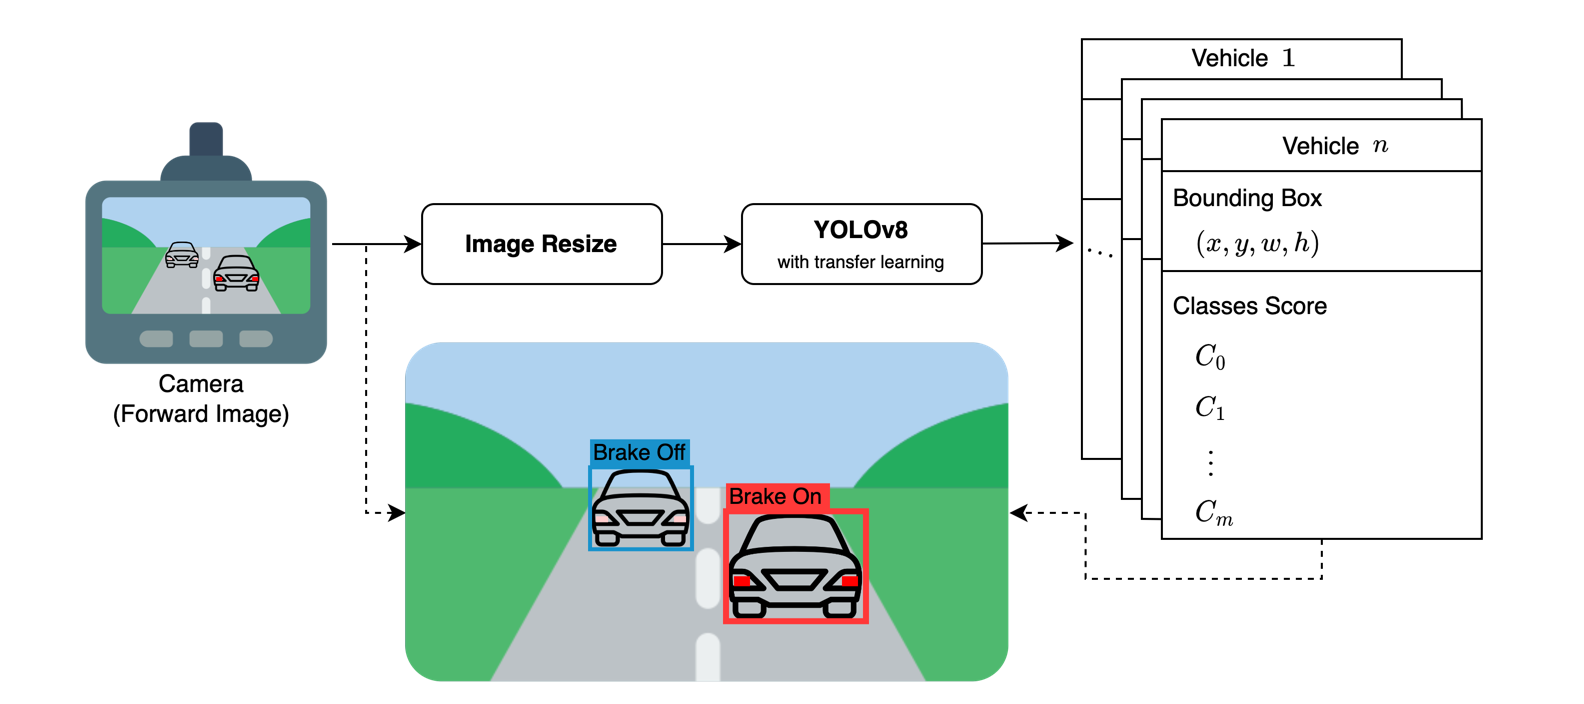
\includegraphics[scale=0.5]{fig/workflow.png}
    \caption{Workflow of the proposed one-stage brake light detection network. The solid line arrows represent the flow of data for inference purposes, while the dashed line arrows represent the flow of data for visualization purposes.}
    \label{fig:workflow}
\end{figure}

In this paper, we propose a one-stage neural network that detects brake lights of preceding vehicles, taking into account the trade-off between inference time and accurate detection performance. 
The proposed network is based on YOLOv8 \cite{YOLOv8}, the latest version of the popular one-stage object detection network, and leverages transfer learning to perform the task of detecting driving vehicles and brake lights as shown in Figure \ref{fig:workflow}.
Existing research on brake light detection utilizing computer vision or artificial neural network techniques exists, but they typically employ multi-stage architectures of two or more stages, neglecting the inference time.

We collected more than 11K real-world driving images and manually annotated the driving vehicle and brake light status for each image for transfer learning with YOLOv8. 
Based on the collected dataset, we conducted transfer learning of YOLOv8 models and evaluated the performance of the models in terms of model size, brake light status, and ambient lighting conditions.
The real-time performance of the trained models was verified using an edge device, Nvidia Jetson Nano, installed in the driving vehicle.
This allowed us to assess the model's ability to make predictions in real-time while considering its computational efficiency.

The main contributions in this study can be described as follows:
\begin{itemize}
    \item We propose a one-stage network for detecting the brake light status of vehicles in the forward image during driving. The proposed network takes a single image as input and outputs bounding boxes for all vehicles present in the image, along with the detection of whether their brake light is on or off. 
    \item We introduce a dataset for the task of driving vehicle and brake light status detection during driving. The dataset consists of over 11K real-world driving images captured under various conditions including day, night, and tunnel. For all the collected image has annotations for vehicle bounding boxes and brake light status, which are manually annotated by experts.
    \item The proposed detection network based on YOLOv8 is fine-tuned using the introduced dataset. The trained model achieve high detection performance and the real-time performance of the model on an edge-device is verified.
\end{itemize}

The rest of this paper is organized as follows. 
Section \ref{sec:related} introduces related works on the general object detection algorithm and brake light status detection. 
Section \ref{sec:proposed} discusses the proposed detection network and dataset for the transfer learning.
Section \ref{sec:experiments} presents the details of transfer learning and analyzes the evaluation results.
Section \ref{sec:conclusions} concludes this work and describes further work. 

\section{Related Works}
\label{sec:related}
% This section presents an overview of prior research regarding brake light detection and YOLO.

Research has been conducted on vehicle brake light status detection for various purposes, including collision avoidance and deceleration prediction.
These studies primarily rely on forward images as the brake light's brightness difference serves as the most significant clue. 
Detection methods can be broadly categorized into image processing \cite{thammakaroon2009predictive, chen2015daytime, liu2015vision}, frequency-tuned \cite{chen2012frequency}, machine learning \cite{cui2015vision, nava2019collision, pirhonen2022brake}, and deep learning approaches \cite{wang2016appearance, li2020highly, kim2022detecting}.
In terms of research scope, most studies focus on daytime conditions \cite{liu2015vision,chen2015daytime,cui2015vision,wang2016appearance,nava2019collision,pirhonen2022brake}, targeting scenarios where the detection of brake light status is relatively straightforward. 
However, there are also studies that address more challenging scenarios, such as nighttime \cite{thammakaroon2009predictive,chen2012frequency} or tunnel environments \cite{kim2022detecting}, where the detection becomes more difficult due to potential confusion with tail lights.
It is less common to find studies that simultaneously address both day- and nighttime conditions \cite{li2020highly}.

Studies that utilize image processing techniques employ heuristic approaches and leverage different color spaces for brake light detection.
Liu et al. utilize the the most common red-green-blue (RGB) color space and apply a threshold for color difference between adjacent frames to detect brake light operation \cite{liu2015vision}.
Similarly, Thammakaroon and Tangamchit also use a threshold in the RGB space, but they additionally perform low light image processing in the hue-saturation-intensity (HSI) color space, focusing on detecting brake light operation in nighttime images \cite{thammakaroon2009predictive}.
Chen et al. utilize a* component in the LAB color space to perform binary thresholding for brake light detection \cite{chen2015daytime}.
In the LAB color space, L* represents the lightness, while a* and b* represent the color ranges, with a* representing the red-green axis and b* representing the yellow-blue axis.
These different color spaces are also utilized in the image preprocessing stages of studies that employ machine learning or deep learning approaches.
Cui et al. use the hue-saturation-value (HSV) color space \cite{cui2015vision}, while Nava et al. and Pirhonen et al. utilize the LAB color space \cite{nava2019collision, pirhonen2022brake}.

In contrast to the heuristic approaches mentioned earlier, Chen and Peng focused on finding invariant features in the frequency domain, presenting an effective methodology for an extensive datasets \cite{chen2012frequency}.
However, in recent years, learning-based methods have shown much more effective performance, leading to extensive research on brake light detection based on machine learning or deep learning techniques.
Cui et al. and Nava et al. achieved high brake light detection performance using support vector machines (SVM), with a $75\%$ detection rate and an F1 score of $0.95$, respectively \cite{cui2015vision, nava2019collision}. 
Pirhonen et al. achieved an accuracy of $82\%$ using the random forest, primarily focusing on objects at distances of $50$ meters or more \cite{pirhonen2022brake}.
Wang et al. utilized deep learning methods, specifically convolutional neural networks (CNN), as the foundation for detecting brake light status and other related features \cite{wang2016appearance}.
They used a pre-trained AlexNet model \cite{krizhevsky2012imagenet} from the ImageNet dataset \cite{russakovsky2015imagenet}, and achieved an accuracy of $89\%$.
Kim utilized not only CNN but also long short-term memory (LSTM) to detect the brake light status of driving vehicles, achieving an accuracy of $90.2\%$ specifically for vehicles driving inside tunnels \cite{kim2022detecting}.
While these machine learning and deep learning methods demonstrated high performance, it is important to note that they all have limitations in that they primarily consider specific scenarios such as daytime or tunnels.
Additionally, they have been validated only on their own nonpublic datasets.

A common limitation among all the mentioned brake light detection studies is the use of a multi-stage detection structure.
These methods all assume that the target vehicle has been detected beforehand, and then the detection of the brake light is performed.
Various methods are used for target vehicle detection, such as the histogram of oriented gradients (HOG) detector \cite{chen2015daytime, wang2016appearance}, combination of HOG detector with SVM \cite{cui2015vision}, and AdaBoost \cite{liu2015vision, freund1996experiments}.
Additionally, initial versions of YOLO \cite{redmon2016you, redmon2017yolo9000} and improved versions like YOLOv3 \cite{redmon2018yolov3} and YOLOv4 \cite{bochkovskiy2020yolov4} are employed for driving vehicle detection \cite{pirhonen2022brake, kim2022detecting}.
Accurate detection of driving vehicles can enhance the performance of brake light status detection. 
However, the multi-stage approach has a significant limitation in terms of real-time capability. 
The fundamental purpose of brake light status detection is to contribute to the development of safer systems by integrating with ADAS or autonomous driving systems. If real-time performance is not ensured, even highly accurate detection loses its value.

Li et al. proposed a one-stage detector for real-time brake light status detection \cite{li2020highly}. 
They utilized a light version of YOLOv3, called YOLOv3-tiny, as the backbone network, and enhanced the detection performance by adding output layers and spatial pyramid pooling (SPP \cite{he2015spatial}). 
They reported a detection performance of mAP $89.13$ for brake activation detection and achieved real-time capability with a frame rate of $63$ FPS.
However, it's important to note that the reported frame rate was measured on a powerful GPU (GTX-1060), which is significantly more powerful than the hardware typically used in real-world vehicle control systems. 
Therefore, it is necessary to propose brake light status detection models that can achieve high detection performance with fast inference speed on the edge devices, which are commonly used in real-world vehicle control systems.




\section{Proposed Work}
\label{sec:proposed}

In this study, we propose a one-stage brake light detection network based on YOLOv8. The network is designed to detect both the driving vehicle and its brake light status in a single stage. 
The input to the network is a single forward image captured from the ego-vehicle, and the outputs consist of the brake light status categories and 2D bounding boxes for all driving vehicles present in the input image (as depicted in in Figure \ref{fig:workflow}).
The 2D bounding box is represented by four numerical values: $x$, $y$, $w$, and $h$. The coordinates $(x,y)$ represent the center of the bounding box, while $w$ and $h$ denote the width and height of the bounding box, respectively. 
The number of classes, denoted as $m$, is defined as $2$, including the brake light status categories.
The classes score, denoted as $C$, represent the probability value associated with each category:

\begin{equation}
    m=2, \;\;\; C   \begin{cases}
        C_{1}=1.0 & \text{ If the brake light is turned off } \\
        C_{2}=1.0 & \text{ If the brake light is turned on }
        \end{cases}
        , \quad w.r.t \sum_{i=1}^{m}{C_{i}}=1.0
\end{equation}

where $C_{1}$ is the probability that the brake light is turned off, and $C_{2}$ is the probability that the brake light is turned on of the detected vehicle.
Hence, the proposed network outputs the bounding boxes for the target vehicles present in the input image, along with the corresponding probability values for the two defined classes.
The target vehicles include conventional passenger cars as well as motorcycles, buses, trucks, and special vehicles.
Only the vehicles with two or more functional brake lights on both the left and right sides of their rear end are taken into consideration as target vehicles.

\subsection{Dataset}
\label{sec:method_dataset}
To accomplish the specific task of detecting brake light status along with the vehicle, a custom dataset needs to be prepared.
The process of creating a custom dataset involves collecting input images and annotating them accordingly.
To collect forward images of the driving vehicle, we utilize a dashboard camera specifically designed to capture video footage of the road ahead during driving. 
We employ two different cameras, namely the FINEVu GX2000 and Mercedes-Benz dashcam, which are mounted on the windshields of different vehicles.
After driving with the vehicle equipped with the dashboard camera, we extract single images from the recorded video.
However, considering that the dashboard camera typically captures more than 30 images per second, using every single image as input for the dataset would result in a large number of similar images.
To address this issue and prevent redundancy in the dataset, we collect the input images at $T$-second intervals from the video.

Another crucial aspect to consider when utilizing dashboard camera images is the camera's image postprocessing capabilities.
Dashboard camera often include features like brightness correction and High Dynamic Range (HDR) to capture clear details, especially in critical situations such as car accidents.
However, it is essential to account for the preprocessing of input data in training a network that can deliver reliable performance even with a general camera lacking image postprocessing features. 
The data preprocessing methods we consider are described in Section \ref{sec:exp_pre}.

\begin{figure}[b!]%

    \subfloat[Light reflection from LED lights]{{\includegraphics[height=3.85cm]{fig/003202.jpg} }}%
    \subfloat[Confusion with tail lights]{{\includegraphics[height=3.85cm]{fig/000117.jpg} }}%
    \hfill
    \subfloat[Preceding image of (a)]{{\includegraphics[height=3.85cm]{fig/003201.jpg} }}%
    \subfloat[Preceding image of (b)]{{\includegraphics[height=3.85cm]{fig/000116.jpg} }}%

\caption{Illustrative cases in which it is difficult to determine the operation of brake lights based on single image} 
% (a) Light reflection from LED lights. (b) Confusion with tail lights. (c) Preceding image of light reflection case. (d) Preceding image of confusion with tail light case}
\label{fig:label_hard}%
\end{figure}

For supervised transfer learning, annotation information in the same format as the output of the proposed network is required.
Six annotation experts manually label information such as the bounding box ($x, y, w, h$) and brake light status ($C$) of vehicles appearing in each collected image.
The experts employ the widely used open-source image annotation tool called LabelImg.
This tool has become part of the open-source data labeling tool, Label Studio \cite{Label_Studio}, which provides more flexible functionalities.
There are several factors that make it challenging for trained experts to annotate from a single image, even with the assistance of useful tools.
One prominent challenge is the presence of light reflection from Light Emitting Diode (LED) lights and confusion with tail lights.
Since most vehicle brake lights are composed of LED lights, they can easily reflect ambient light.
Consequently, when ambient light is reflected from an LED light and reaches the camera, the LED itself may appear to emit light even if it is not turned on.
This illusion creates difficulty in determining whether the brake light of a vehicle is turned on or off.
Figure \ref{fig:label_hard}-(a) illustrates a scenario where it is challenging to discern the brake light status of the vehicle in the center of the image due to the bright surrounding light. 
Even when comparing the light intensity of the vehicle on the left side of the image, where the brake light is turned on, with the vehicle on the right side of the image, where the brake light is turned off, it shows an intermediate level.
While the light reflection is more prevalent during the daytime when there is ample ambient light, confusion with tail lights arises at night.
Figure \ref{fig:label_hard}-(b) showcases a scenario where it is difficult to determine whether the vehicle in the center of the image has only the tail light of both the tail light and brake light is turned on.
This confusion becomes more pronounced when there are no surrounding vehicles in the image.
To overcome these challenges, the experts annotate by referring to several preceding or succeeding images. 
Figure \ref{fig:label_hard}-(c) and (d) depict preceding images captured in close proximity to Figure \ref{fig:label_hard}-(a) and (b), respectively.
By referring to the preceding images, it becomes much easier to determine whether the brake lights of the vehicles in Figure \ref{fig:label_hard}-(a) and (b) are turned on.

The details of the dataset are described in Section \ref{sec:exp_pre}, and the train dataset is publicly available for access \cite{brake-light-detection_dataset}.



\subsection{YOLOv8}
YOLO, which stands for ``You Only Look Once,'' is a well-known multi-object detection algorithms \cite{redmon2016you}.
As its name suggests, YOLO aims to provide detection results by analyzing the image only once. 
Prior to the introduction of YOLO, many multi-object detection algorithms relied on multiple stages to accurately detect object location and class \cite{girshick2014rich, he2015spatial, girshick2015fast, ren2015faster}.
However, these approaches had limitations in real-time applications due to the need for multiple steps.
YOLO revolutionized object detection by simultaneously detecting the locations and classes of objects using a single neural network.
Since its inception, YOLO has been recognized for its fast inference speed and high accuracy compared to other object detection algorithms.
It has evolved from YOLOv1 to latest state-of-the-art version, YOLOv8 \cite{redmon2016you, redmon2017yolo9000, redmon2018yolov3, bochkovskiy2020yolov4, YOLOv5, li2022yolov6, wang2023yolov7, YOLOv8}.
YOLO has extended its capabilities beyond its original task of detecting $80$ objects defined by MS-COCO \cite{lin2014microsoft} and has been widely utilized as a backbone or benchmarking model in various detection fields, including remote sensing \cite{ye2022adaptive} and tiny defects detection \cite{zeng2022small}.
It has provided significant research inspiration across different domains.
Therefore, in this study, we propose a network based on the YOLOv8, the latest state-of-the-art one-stage multi-object detection algorithm, to detect driving vehicle on the road and their brake light status, building upon the rich foundation of YOLO's achievements in diverse detection tasks.

YOLOv8 \cite{YOLOv8} was officially released in January 2023 and incorporates updates from YOLOv5 \cite{YOLOv5}.
Notable updates in YOLOv8 include a structural changes in the partial bottleneck, a shift to an anchor-free approach with the decoupled head, and a change in the activation function of the top layer \cite{terven2023comprehensive}.
The loss functions utilized in YOLOv8 include binary cross-entropy for classification loss, complete intersection over union (CIoU) \cite{zheng2020distance}, and distribution focal loss (DFL) \cite{li2020generalized} for localization loss.
The output of the proposed network consists of $8,400$ bounding boxes, with $6$ parameters assigned to each input image.
These parameters represent the 2D center coordinates, width, and height of the bounding box ($x, y, w, h$), as well as the probability values for each class, indicating whether the brake light is turned off or on. 
Among the $8,400$ output bounding boxes, postprocessing techniques such as non-maximum suppression (NMS) are employed to filter out insignificant detections.
This helps eliminate redundant and overlapping bounding boxes, resulting in a more refined and accurate set of detections.



\section{Experiments}
\label{sec:experiments}

The experimental evaluation of the proposed method is presented in this section. 
Section \ref{sec:exp_pre} provides details about the custom dataset collected as described in Section \ref{sec:proposed}, as well as preprocessing steps.
Section \ref{sec:exp_transfer} focuses on the transfer learning process of YOLOv8 using the custom dataset.
The experimental results are presented in detail in Section \ref{sec:exp_results}.

\subsection{Custom dataset \& Preprocessing}
\label{sec:exp_pre}
A large-scale custom dataset consisting over 16 hours of data was collected. 
Videos recorded from dashboard cameras during real road driving were utilized, resulting in a total of more than $11,000$ images.
These images were obtained by setting the time interval $T$ to $5$ seconds.
Manual annotation was performed on all images to label the bounding box of the driving vehicle and the brake light status of each vehicle.
The total number of annotations exceeded $30,000$.
To ensure a balanced and diverse dataset, various driving scenarios were included, such as daytime, nighttime, city, highway, and tunnel environments.
Precautions were taken to avoid bias toward any specific category, ensuring information about the number of images and annotations in the train and test sets for each category of brake light status.
The details of numbers of images and annotations in the train and test sets in each category of brake light status are given in Table \ref{tab:dataset}.

\begin{table}[h]
    \caption{Details of train and test datasets}
    \label{tab:dataset}
    % \resizebox{\textwidth*0.5}{!}{%
    \begin{tabular}{p{5cm} p{5cm} p{5cm}}
        % {lrr}
    \toprule
    \multicolumn{1}{c}{Number of}                          & \multicolumn{1}{c}{Train} & \multicolumn{1}{c}{Test} \\
    \midrule
    Images                              & \multicolumn{1}{r}{7,892}                     & \multicolumn{1}{r}{3,196}                    \\
    Annotations                         & \multicolumn{1}{r}{19,913}                    & \multicolumn{1}{r}{10,531}                   \\
    \multicolumn{1}{c}{Brake Light Off ($C_{1}=1.0$)} & \multicolumn{1}{r}{10,851}                    & \multicolumn{1}{r}{5,999}                    \\
    \multicolumn{1}{c}{Brake Light On ($C_{2}=1.0$)}  & \multicolumn{1}{r}{9,062}                     & \multicolumn{1}{r}{4,532}                   \\
    \bottomrule
    \end{tabular}%
    % }
\end{table}





To make our custom dataset trainable with YOLOv8 and achieve robust performance, several preprocessing steps are necessary.
The first crucial processes involve image resizing and normalization.
In order to maintain a consistent input size, the width and height of all images were resized to $I_{w}$ and $I_{h}$, respectively. 
In this study, both $I_{w}$ and $I_{h}$ were defined as $640$.
Regarding image normalization, min-max normalization was applied to normalize the pixel values.
The normalization precess ensure that all pixel values fall within a specific range, typically between $0$ and $1$, and is performed as follows:

\begin{figure}[b!]%

    \subfloat[Reshape]{{\includegraphics[height=3.4cm]{fig/preprocessing_reshape.jpeg} }}%
    \subfloat[horizontal flip]{{\includegraphics[height=3.4cm]{fig/preprocessing_flip.jpeg} }}%
    \subfloat[Crop]{{\includegraphics[height=3.4cm]{fig/preprocessing_crop.jpeg} }}%
    \subfloat[Black-box cutout]{{\includegraphics[height=3.4cm]{fig/preprocessing_cutout.jpeg} }}%
    \hfill
    \subfloat[Brightness increase]{{\includegraphics[height=3.4cm]{fig/preprocessing_brightness_max.jpeg} }}%
    \subfloat[Brightness decrease]{{\includegraphics[height=3.4cm]{fig/preprocessing_brightness_min.jpeg} }}%
    \subfloat[Blur]{{\includegraphics[height=3.4cm]{fig/preprocessing_blur} }}%
    \subfloat[Noise]{{\includegraphics[height=3.4cm]{fig/preprocessing_noise.jpeg} }}%

\caption{Examples of individual random modifications applied during the preprocessing stage. (c) to (n) represent example images that reflect the maximum extent of each random modification considered.}
\label{fig:random}%
\end{figure}

\begin{equation}
    x_{norm} = \frac{x - x_{min}}{x_{max} - x_{min}}
\end{equation}
where $x$ and $x_{norm}$ are origin and normalized pixel value, respectively and $x_{max}$ and $x_{min}$ are the maximum and minimum pixel value of the image, respectively.
In this study, the values for $x_{max}$ and $x_{min}$ were set to $255.0$ and $0.0$, respectively, following the usual convention.
Furthermore, various data augmentation techniques were applied to enhance the robustness of the inference performance.
Random horizontal flipping and image cropping were performed to generate variations of the collected images that could realistically occur.
To improve detection performance in cases of occlusion, random black-box cutout augmentation was also applied.
Finally, to ensure robustness across different camera setups, the quality of the input images was intentionally degraded using various methods.
As stated in Section \ref{sec:method_dataset}, the dashboard cameras used for image acquisition are equipped with various postprocessing methods to captured high-quality images.
To ensure the robust performance of the trained network even with general cameras, random modifications such as brightness changes, blur, and noise injection were applied to the images.
The details of all random modifications applied during the preprocessing stage are as follows:

\begin{figure}[b!]%

    \subfloat{{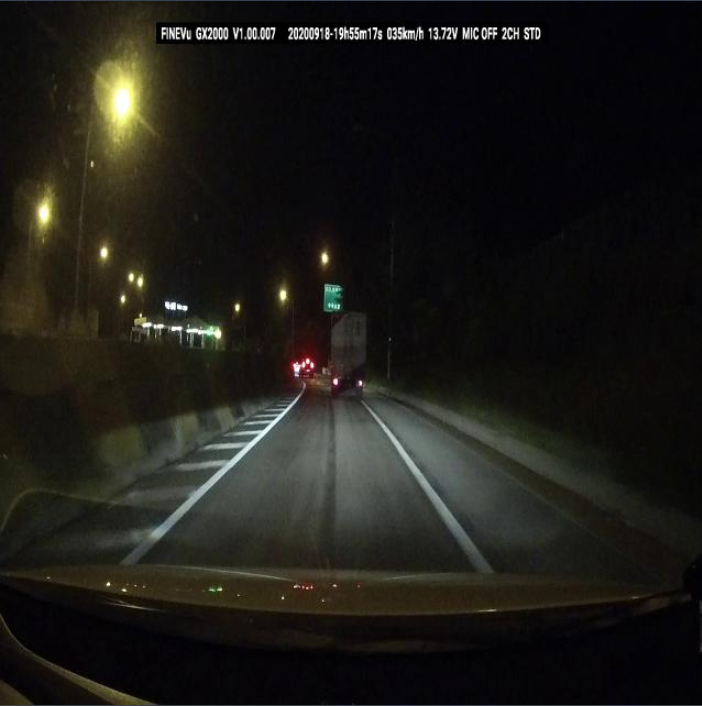
\includegraphics[height=4.5cm]{fig/image20.png} }}%
    \subfloat{{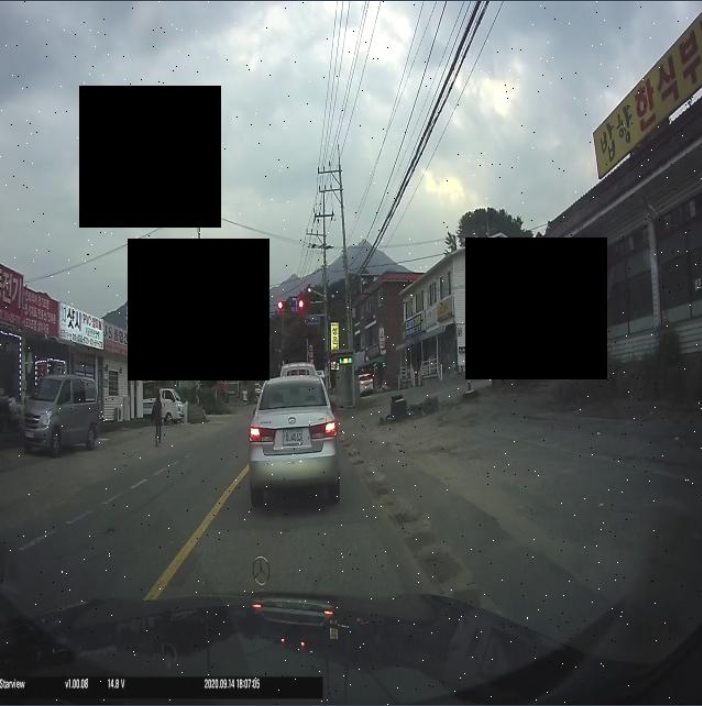
\includegraphics[height=4.5cm]{fig/image21.png} }}%
    \subfloat{{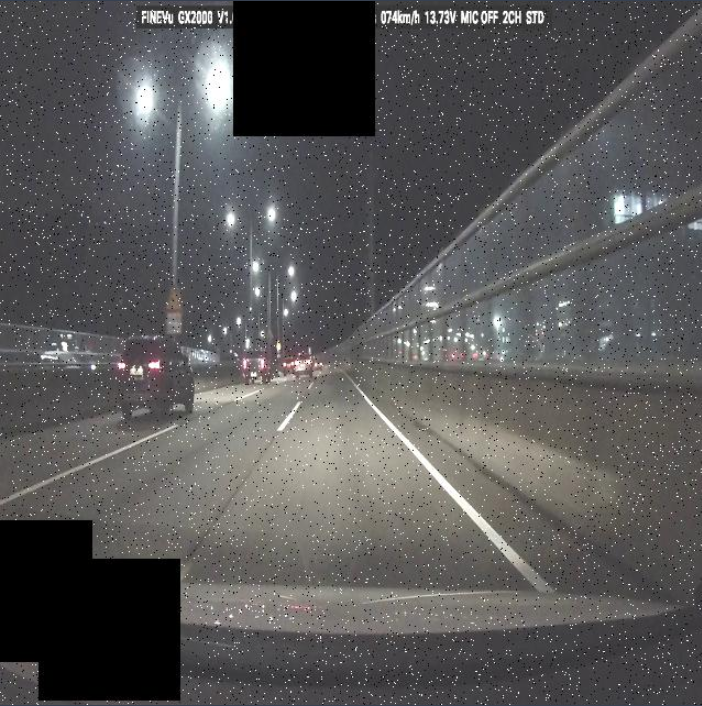
\includegraphics[height=4.5cm]{fig/image22.png} }}%
    \hfill
    \subfloat{{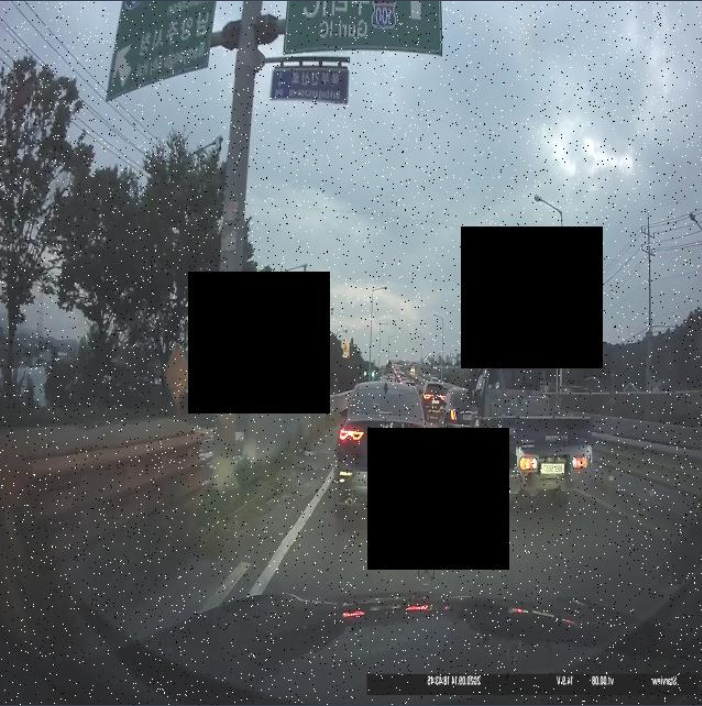
\includegraphics[height=4.5cm]{fig/image23.png} }}%
    \subfloat{{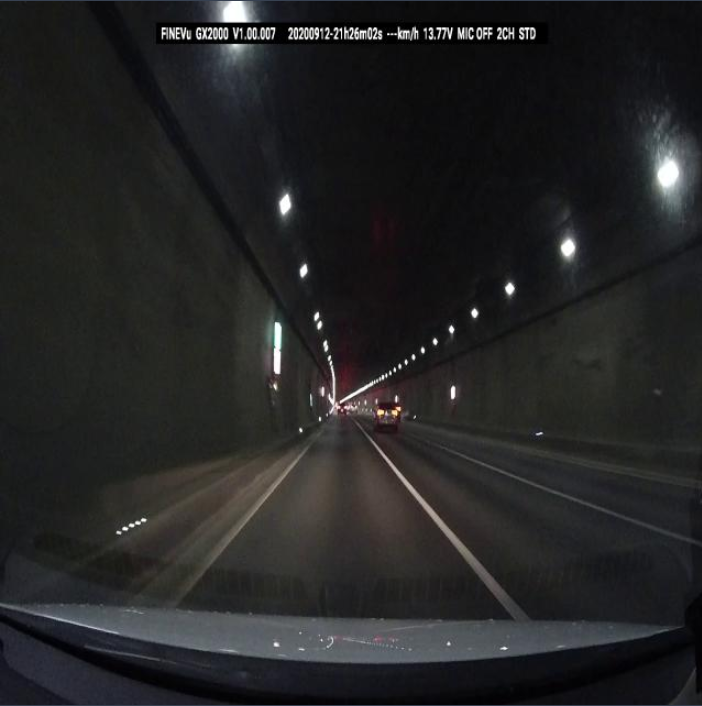
\includegraphics[height=4.5cm]{fig/image24.png} }}%
    \subfloat{{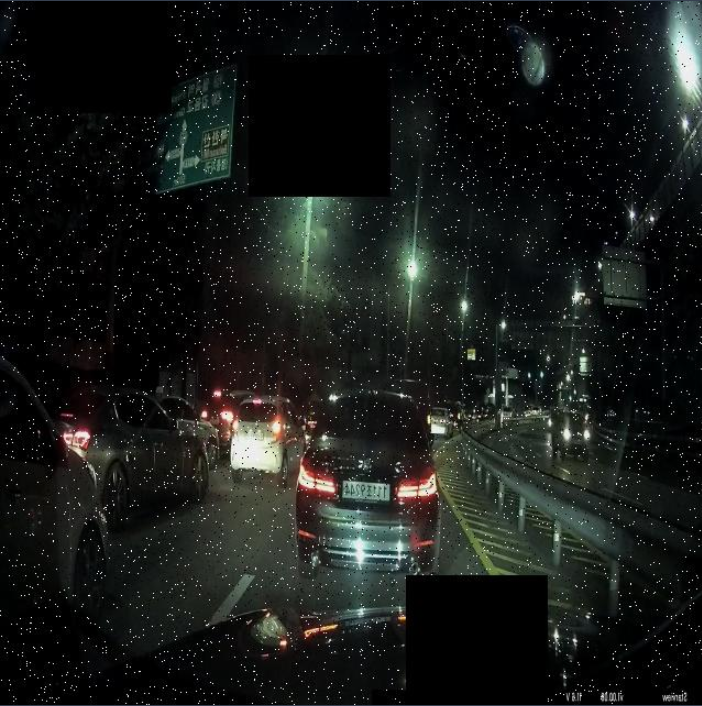
\includegraphics[height=4.5cm]{fig/image25.png} }}%

\caption{Preprocessed input images of custom dataset}
\label{fig:custom_dataset}%
\end{figure}

\begin{itemize}
    \item{Crop: zoom rate chosen from uniform distribution within the range of $0\%$ to $20\%$}
    \item{Cutout: a maximum size of black-box is $20\%$ of image size, a maximum of $3$ boxes}
    \item{Brightness: adjustment with a range of minimum $-25\%$ to maximum $+25\%$}
    \item{Blur: a gaussian blur with a maximum kernel size of $3 \times 3$}
    \item{Noise: add noise to a maximum of $5\%$ of pixels}
\end{itemize}
The images illustrating each modification can be found in Figure \ref{fig:random}.
Figure \ref{fig:custom_dataset} provides examples of preprocessed images.
All preprocessing steps were performed using Roboflow \cite{roboflow}, a comprehensive platform for computer vision and image processing tasks.
The preprocessed train dataset is publicly available for access \cite{brake-light-detection_dataset}.




\subsection{Transfer learning}
\label{sec:exp_transfer}
In this study, we conducted transfer learning on all models provided by YOLOv8 \cite{YOLOv8} to develop a detection network that achieves real-time inference in a driving vehicle while maintaining accurate detection.
The YOLOv8 architecture offers five different models of varying sizes, ranging from the smallest model (YOLOv8n) to the largest model (YOLOv8x), as shown in Table \ref{tab:yolov8}.
To ensure consistency, the same set of hyperparameters was applied to all models during training.
A random 20\% of the train dataset was set aside as the validation dataset for monitoring the training progress.
The initial parameter values for each model were obtained from the pretrained parameters officially provided by YOLOv8.
The training process consisted fo $300$ iterations, with a patience value of $20$.
If there was no observable improvement in the validation loss over the most recent $20$ iterations, the training was terminated early to save time and resources.
Stochastic gradient descent (SGD) optimizer with a learning rate of $0.01$ was used, incorporating both momentum and Nesterov Accelerated Gradient (NAG) techniques \cite{sutskever2013importance} with a momentum coefficient of $0.937$.
The training loss was calculated using three loss function: binary cross-entropy, CIoU, and DFL.
The weighting factors assigned th these loss functions were $0.5$, $7.5$, and $1.5$, respectively.
These factors were chosen to balance the impact of each loss function during training.

\begin{table}[h]
    \caption{Official deployed models of YOLOv8}
    \label{tab:yolov8}
    % \resizebox{\textwidth}{!}{%
    \begin{tabular}{lcc}
    \toprule
    \multicolumn{1}{c}{Model}   & \# params (M) & FLOPs (B) \\
    \midrule
    YOLOv8n & 3.2        & 8.7       \\
    YOLOv8s & 11.2       & 28.6      \\
    YOLOv8m & 25.9       & 78.9      \\
    YOLOv8l & 43.7       & 165.2     \\
    YOLOv8x & 68.2       & 257.8     \\
    \bottomrule
    \multicolumn{3}{l}{\textit{Note:} All values in the table correspond}\\
    \multicolumn{3}{l}{\qquad \; to an input image size of 640x640.}
    \end{tabular}%
    % }
\end{table}

\begin{figure}[t]%
    \captionsetup[subfigure]{justification=centering}

    \subfloat[]{{\includegraphics[height=1.9cm]{fig/img/2-1.jpg} }}%
    \subfloat[]{{\includegraphics[height=1.9cm]{fig/img/2-2.jpg} }}%
    \subfloat[]{{\includegraphics[height=1.9cm]{fig/img/3-1_zoom.png} }}%
    \subfloat[]{{\includegraphics[height=1.9cm]{fig/img/3-2_zoom.png} }}%
    \hfill
    \subfloat[]{{\includegraphics[height=1.9cm]{fig/img/1-1.jpg} }}%
    \subfloat[]{{\includegraphics[height=1.9cm]{fig/img/1-2.jpg} }}%
    \subfloat[]{{\includegraphics[height=1.9cm]{fig/img/1-3.jpg} }}%
    \subfloat[]{{\includegraphics[height=1.9cm]{fig/img/1-4.jpg} }}%
    \hfill
    \subfloat[]{{\includegraphics[height=1.9cm]{fig/img/4-1_zoom.png} }}%
    \subfloat[]{{\includegraphics[height=1.9cm]{fig/img/4-2_zoom.png} }}%
    \subfloat[]{{\includegraphics[height=1.9cm]{fig/img/4-3_zoom.png} }}%
    \subfloat[]{{\includegraphics[height=1.9cm]{fig/img/4-4_zoom.png} }}%

\caption{Qualitative analysis images of driving vehicle and brake light status detection by proposed networks. (a)-(b) is a continuous image pair showcasing the scenario with leading vehicle at a close distance. (c)-(d) is the continuous image pair showcasing the scenario with leading vehicle at a far distance. (e)-(h) are the continuous image pairs showcasing the scenario with multiple vehicles at a close distance. (i)-(l) are the continuous image pairs showcasing the scenario with multiple vehicles at a far distance.
}
\label{fig:qualitative_perf}%
\end{figure}

\begin{figure}[t!]%
    % \captionsetup[subfigure]{justification=centering}

    \subfloat[Highway]{{\includegraphics[height=1.9cm]{fig/Capture/0_highway.jpg} }}%
    \subfloat[City]{{\includegraphics[height=1.9cm]{fig/Capture/0_city.jpg} }}%
    \subfloat[Tunnel]{{\includegraphics[height=1.9cm]{fig/Capture/0_tunnel.jpg} }}%
    \subfloat[Nighttime]{{\includegraphics[height=1.9cm]{fig/Capture/0_night.jpg} }}%
    \hfill
    \subfloat[Motorcycle]{{\includegraphics[height=1.9cm]{fig/Capture/0_motor.jpg} }}%
    \subfloat[Bus]{{\includegraphics[height=1.9cm]{fig/Capture/0_bus.jpg} }}%
    \subfloat[Truck]{{\includegraphics[height=1.9cm]{fig/Capture/0_truck.jpg} }}%
    \subfloat[Special vehicle]{{\includegraphics[height=1.9cm]{fig/Capture/0_special_1.jpg} }}%

\caption{Qualitative analysis images for various driving environments and vehicle types, mainly intended as examples for the following: (a) Hightway, (b) City, (c) Tunnel, (d) Nighttime, (e) Motorcycle, (f) Bus, (g) Truck, and (h) Special vehicle.
}
\label{fig:qualitative_env}%
\end{figure}




\subsection{Results}
\label{sec:exp_results}
In this section, the evaluation results of the trained detection models are presented, both qualitatively and quantitatively.
Qualitative analysis confirmed that the trained detection models accurately detect the bounding boxes of driving vehicles and classify their brake light status (on or off) in various road environments.
Figure \ref{fig:qualitative_perf} shows some of the images used for qualitative analysis.
These images are provided as pairs of two or more consecutive frames to demonstrate clear analysis results.
(a)-(b) represent one continuous image pair displaying the detection performance of leading vehicle located at a close distance.
(c)-(d) represent another continuous image pair displaying the detection performance of leading vehicle located at a far distance.
As evident from these two image pairs, the proposed model accurately detects the location and brake light status of leading vehicles regardless of their distance from the ego vehicle.
(e)-(h) represent other continuous image pairs depicting scenarios with multiple vehicles present at a close distance.
In these images, the location and brake light status of all vehicles in the images are successfully detected.
Furthermore, even in scenarios with multiple vehicles at a far distance, all vehicles are accurately detected, as demonstrated by images pairs (i)-(l).

Qualitative analysis was conducted not only for different vehicle quantities and distances but also for various driving environments and vehicle types.
Figure \ref{fig:qualitative_env} (a)-(d) demonstrate the robust performance of the trained model in diverse driving environments, including highway, city, tunnel, and nighttime.
Figure \ref{fig:qualitative_env} (e)-(h) provide qualitative evidence that the model has ability to detect various vehicle types, including passenger cars, motorcycles, buses, trucks, and special vehicles.

The evaluation of the driving vehicle and brake light status detection performance of each model that underwent transfer learning is conducted by calculating the mean average precision (mAP) on the testset.
Two mAP values are calculated: mAP50 and mAP50-95.
mAP50 represents the average precision at an intersection over union (IoU) threshold of $0.5$. The IoU threshold measures the overlap between the predicted bounding boxes and the ground truth labels, indicating how well the predicted boxes align with the actual objects.
mAP50-95 represents the average precision over a range of IoU thresholds from $0.5$ to $0.95$, with a step size of $0.05$. 
This metric provides comprehensive assessment of the detection model's performance across different levels of overlap.
Both mAP50 and mAP50-95 are commonly used metrics to evaluate the overall performance of object detection models.

\begin{figure}[t]%

    \subfloat[\centering mAP50 on the entire testset]{{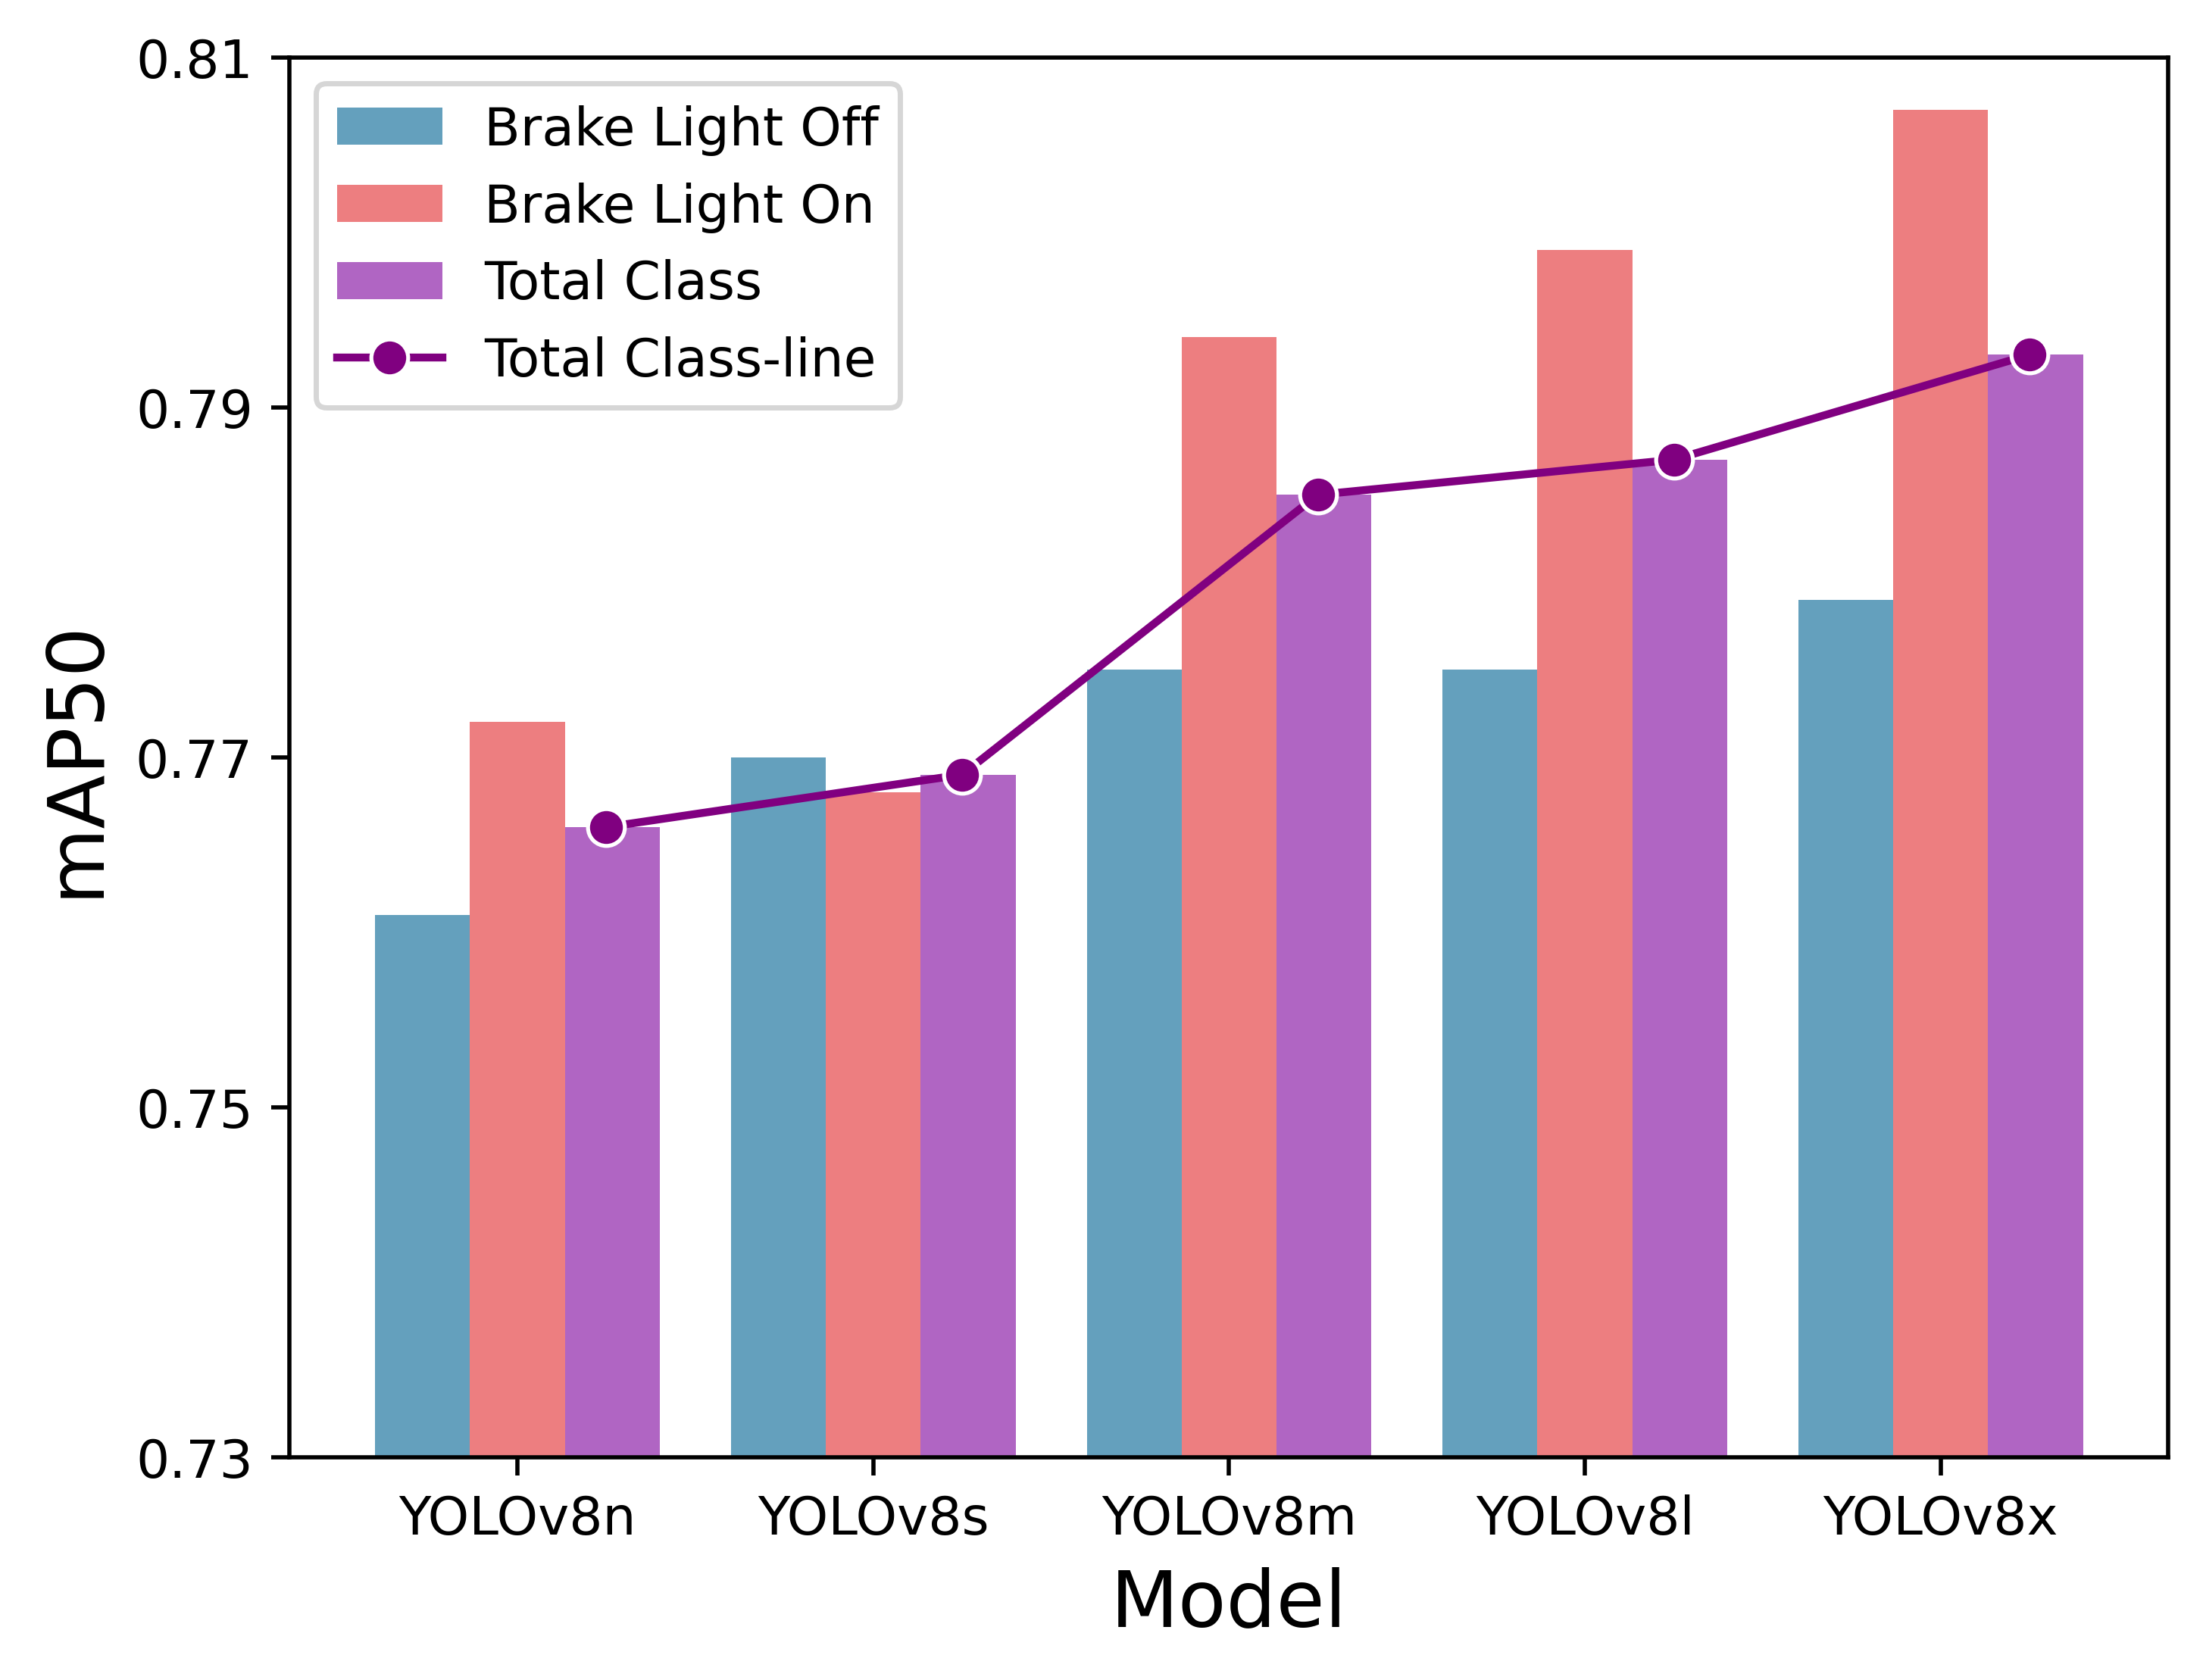
\includegraphics[height=5cm]{fig/bar_map50.png} }}%
    \subfloat[\centering mAP50-95 on the entire testset]{{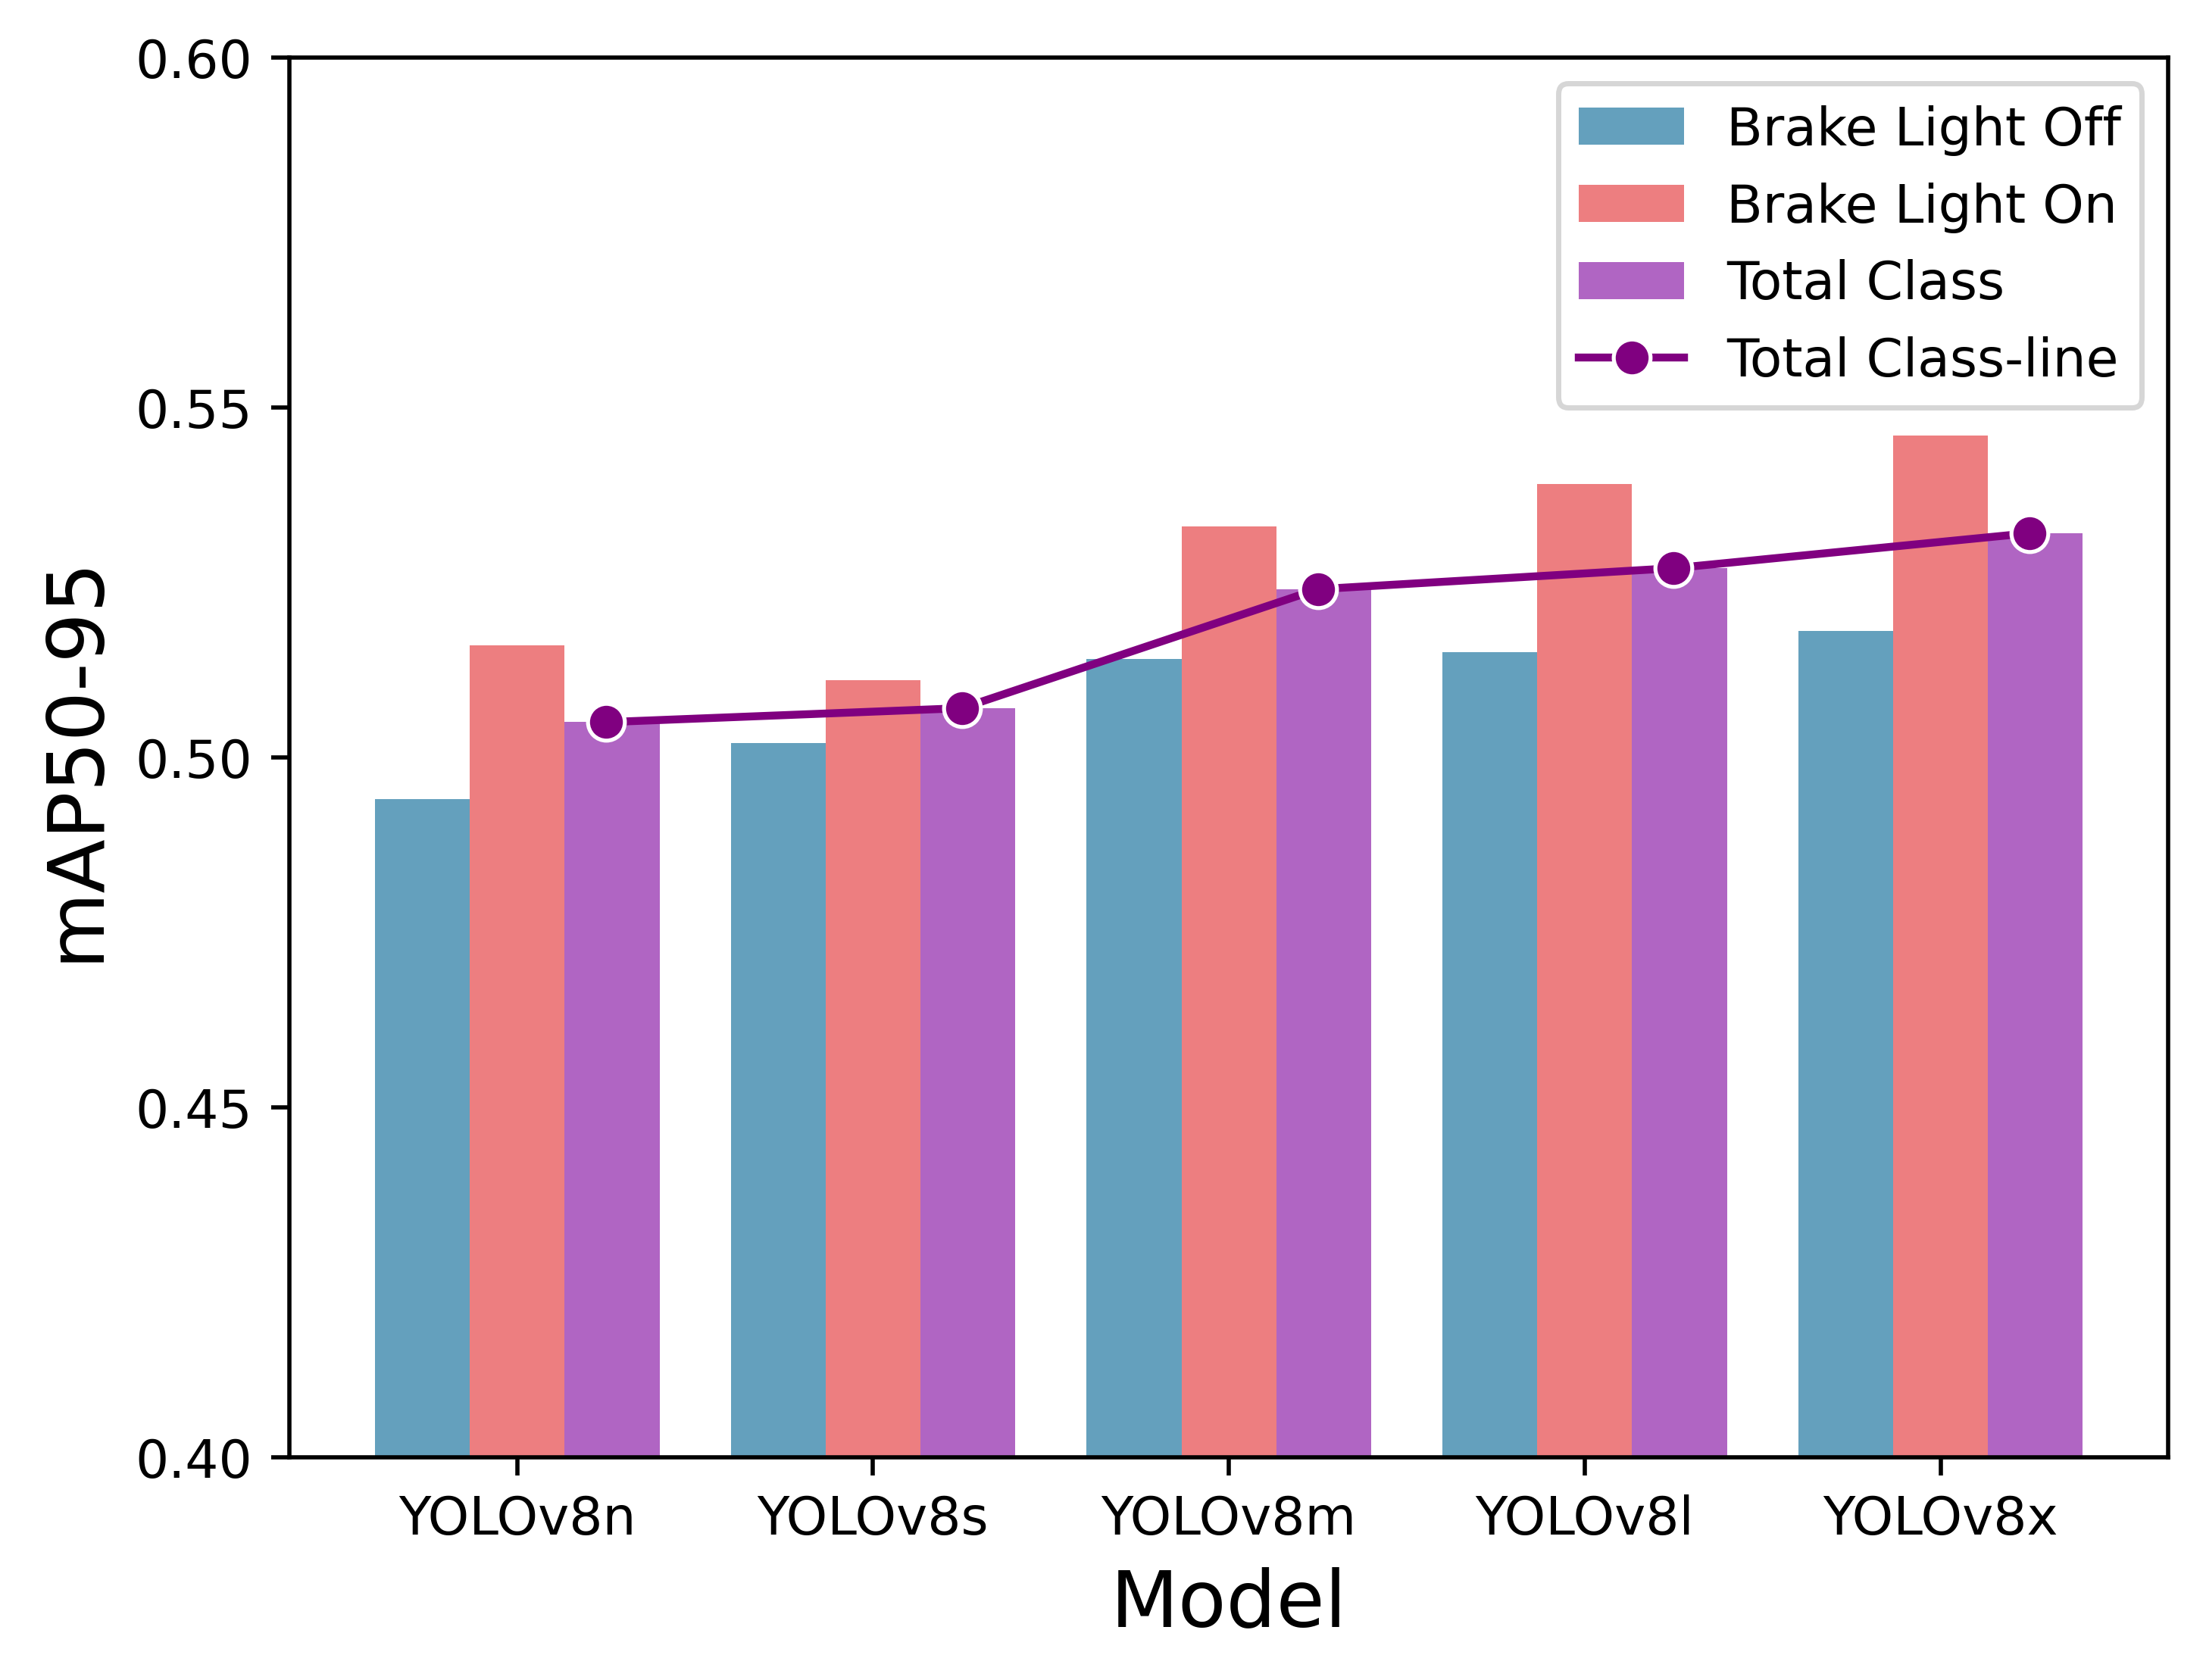
\includegraphics[height=5cm]{fig/bar_map50-95.png} }}%

\caption{Detection performance on the entire testset. The y-axis represents the detection accuracy, and the x-axis lists the YOLOv8 models, with larger models positioned toward the right. Each model is depicted with three bars, showcasing the detection performance for brake light off class, brake light on class, and total class, respectively. Single line plot highlights the difference in detection performance by models for total class.}
\label{fig:test_results}%
\end{figure}

\begin{table}[t!]
    \caption{Results of the entire testset}
    \label{tab:total}
    % \resizebox{\textwidth}{!}{%
    % \begin{tabular}{>{\raggedright}p{2.5cm} >{\raggedright}p{2.5cm} >{\centering}p{2.5cm} >{\centering\arraybackslash}p{2.5cm}}
    \begin{tabular}{llrrrrr}
    \toprule
    \multicolumn{1}{c}{Model} & \multicolumn{1}{c}{Class} & \multicolumn{1}{c}{Precision} & \multicolumn{1}{c}{Recall} & \multicolumn{1}{c}{F1 score} & \multicolumn{1}{c}{mAP50} & \multicolumn{1}{c}{mAP50-95} \\
    \midrule
    \multirow{3}{*}{YOLOv8n}  & Brake Light Off           & 0.726 & 0.670 & 0.697 & 0.761                     & 0.494                          \\
                              & Brake Light On            & 0.549 & 0.853 & 0.668 & 0.772                     & 0.516                        \\
                              & \multicolumn{1}{r}{Total} & 0.638 & 0.762 & 0.695 & 0.766                     & 0.505                        \\
    \midrule
    \multirow{3}{*}{YOLOv8s}  & Brake Light Off           & 0.755 & 0.646 & 0.696 & 0.770                     & 0.502                        \\
                              & Brake Light On            & 0.591 & 0.837 & 0.693 & 0.768                     & 0.511                        \\
                              & \multicolumn{1}{r}{Total} & 0.673 & 0.742 & 0.706 & 0.769                     & 0.507                        \\
    \midrule
    \multirow{3}{*}{YOLOv8m}  & Brake Light Off           & 0.755 & 0.650 & 0.699 & 0.775                     & 0.514                         \\
                              & Brake Light On            & 0.579 & 0.839 & 0.685 & 0.794                     & 0.533                        \\
                              & \multicolumn{1}{r}{Total} & 0.667 & 0.745 & 0.704 & 0.785                     & 0.524                        \\
    \midrule
    \multirow{3}{*}{YOLOv8l}  & Brake Light Off           & 0.746 & 0.655 & 0.698 & 0.775                     & 0.515                         \\
                              & Brake Light On            & 0.552 & 0.867 & 0.675 & 0.799                     & 0.539                        \\
                              & \multicolumn{1}{r}{Total} & 0.649 & 0.761 & 0.701 & 0.787                     & 0.527                      \\
    \midrule
    \multirow{3}{*}{YOLOv8x}  & Brake Light Off           & 0.746 & 0.650 & 0.695 & 0.779                     & 0.518                         \\
                              & Brake Light On            & 0.578 & 0.859 & 0.691 & 0.807                     & 0.546                        \\
                              & \multicolumn{1}{r}{Total} & 0.662 & 0.754 & 0.705 & 0.793                     & 0.532                      \\
    \bottomrule
    \end{tabular}%
    % }
\end{table}

Figure \ref{fig:test_results} presents the detection performance of each trained model, showcasing the results for mAP50 and mAP50-90 in Figure \ref{fig:test_results}-(a) and (b) respectively.
The detection performance for each individual classes, brake light off and brake light on, is represented by blue and red bars respectively. 
The overall detection performance for all classes is shown by the purple bar, with a purple line plot illustrating the trend of performance differences across models.
Both mAP50 and mAP50-95 exhibit similar overall trands, although they differ in scale.
As expected, the detection performance for all classes generally increases as the model size increases.
However, the YOLOv8s model shows a slightly lower performance increase, primarily due to its lower brake light on class detection performance.
Comparing the mAP50 values for each class, it can be observed that all models, except for YOLOv8s, have higher detection performance for the brake light on class compared to the brake light off class.
Overall, the proposed methodology achieved mAP50 values ranging from $0.766$ to $0.793$ and mAP50-95 values ranging from $0.505$ to $0.532$.
Considering the recent benchmarking performance of MS-COCO \cite{lin2014microsoft}, which is one of the leading object detection, with mAP50 values ranging form $71.9$ to $77.0$ and mAP50-95 values ranging from $57.7$ to $58.8$, the proposed methodology demonstrates significant results \cite{coco_benchmark, zou2023object}.
Detailed detection performance for each model and class can be found in Table \ref{tab:total}.

\begin{figure}[b!]%

    \subfloat[mAP50 on the Day testset]{{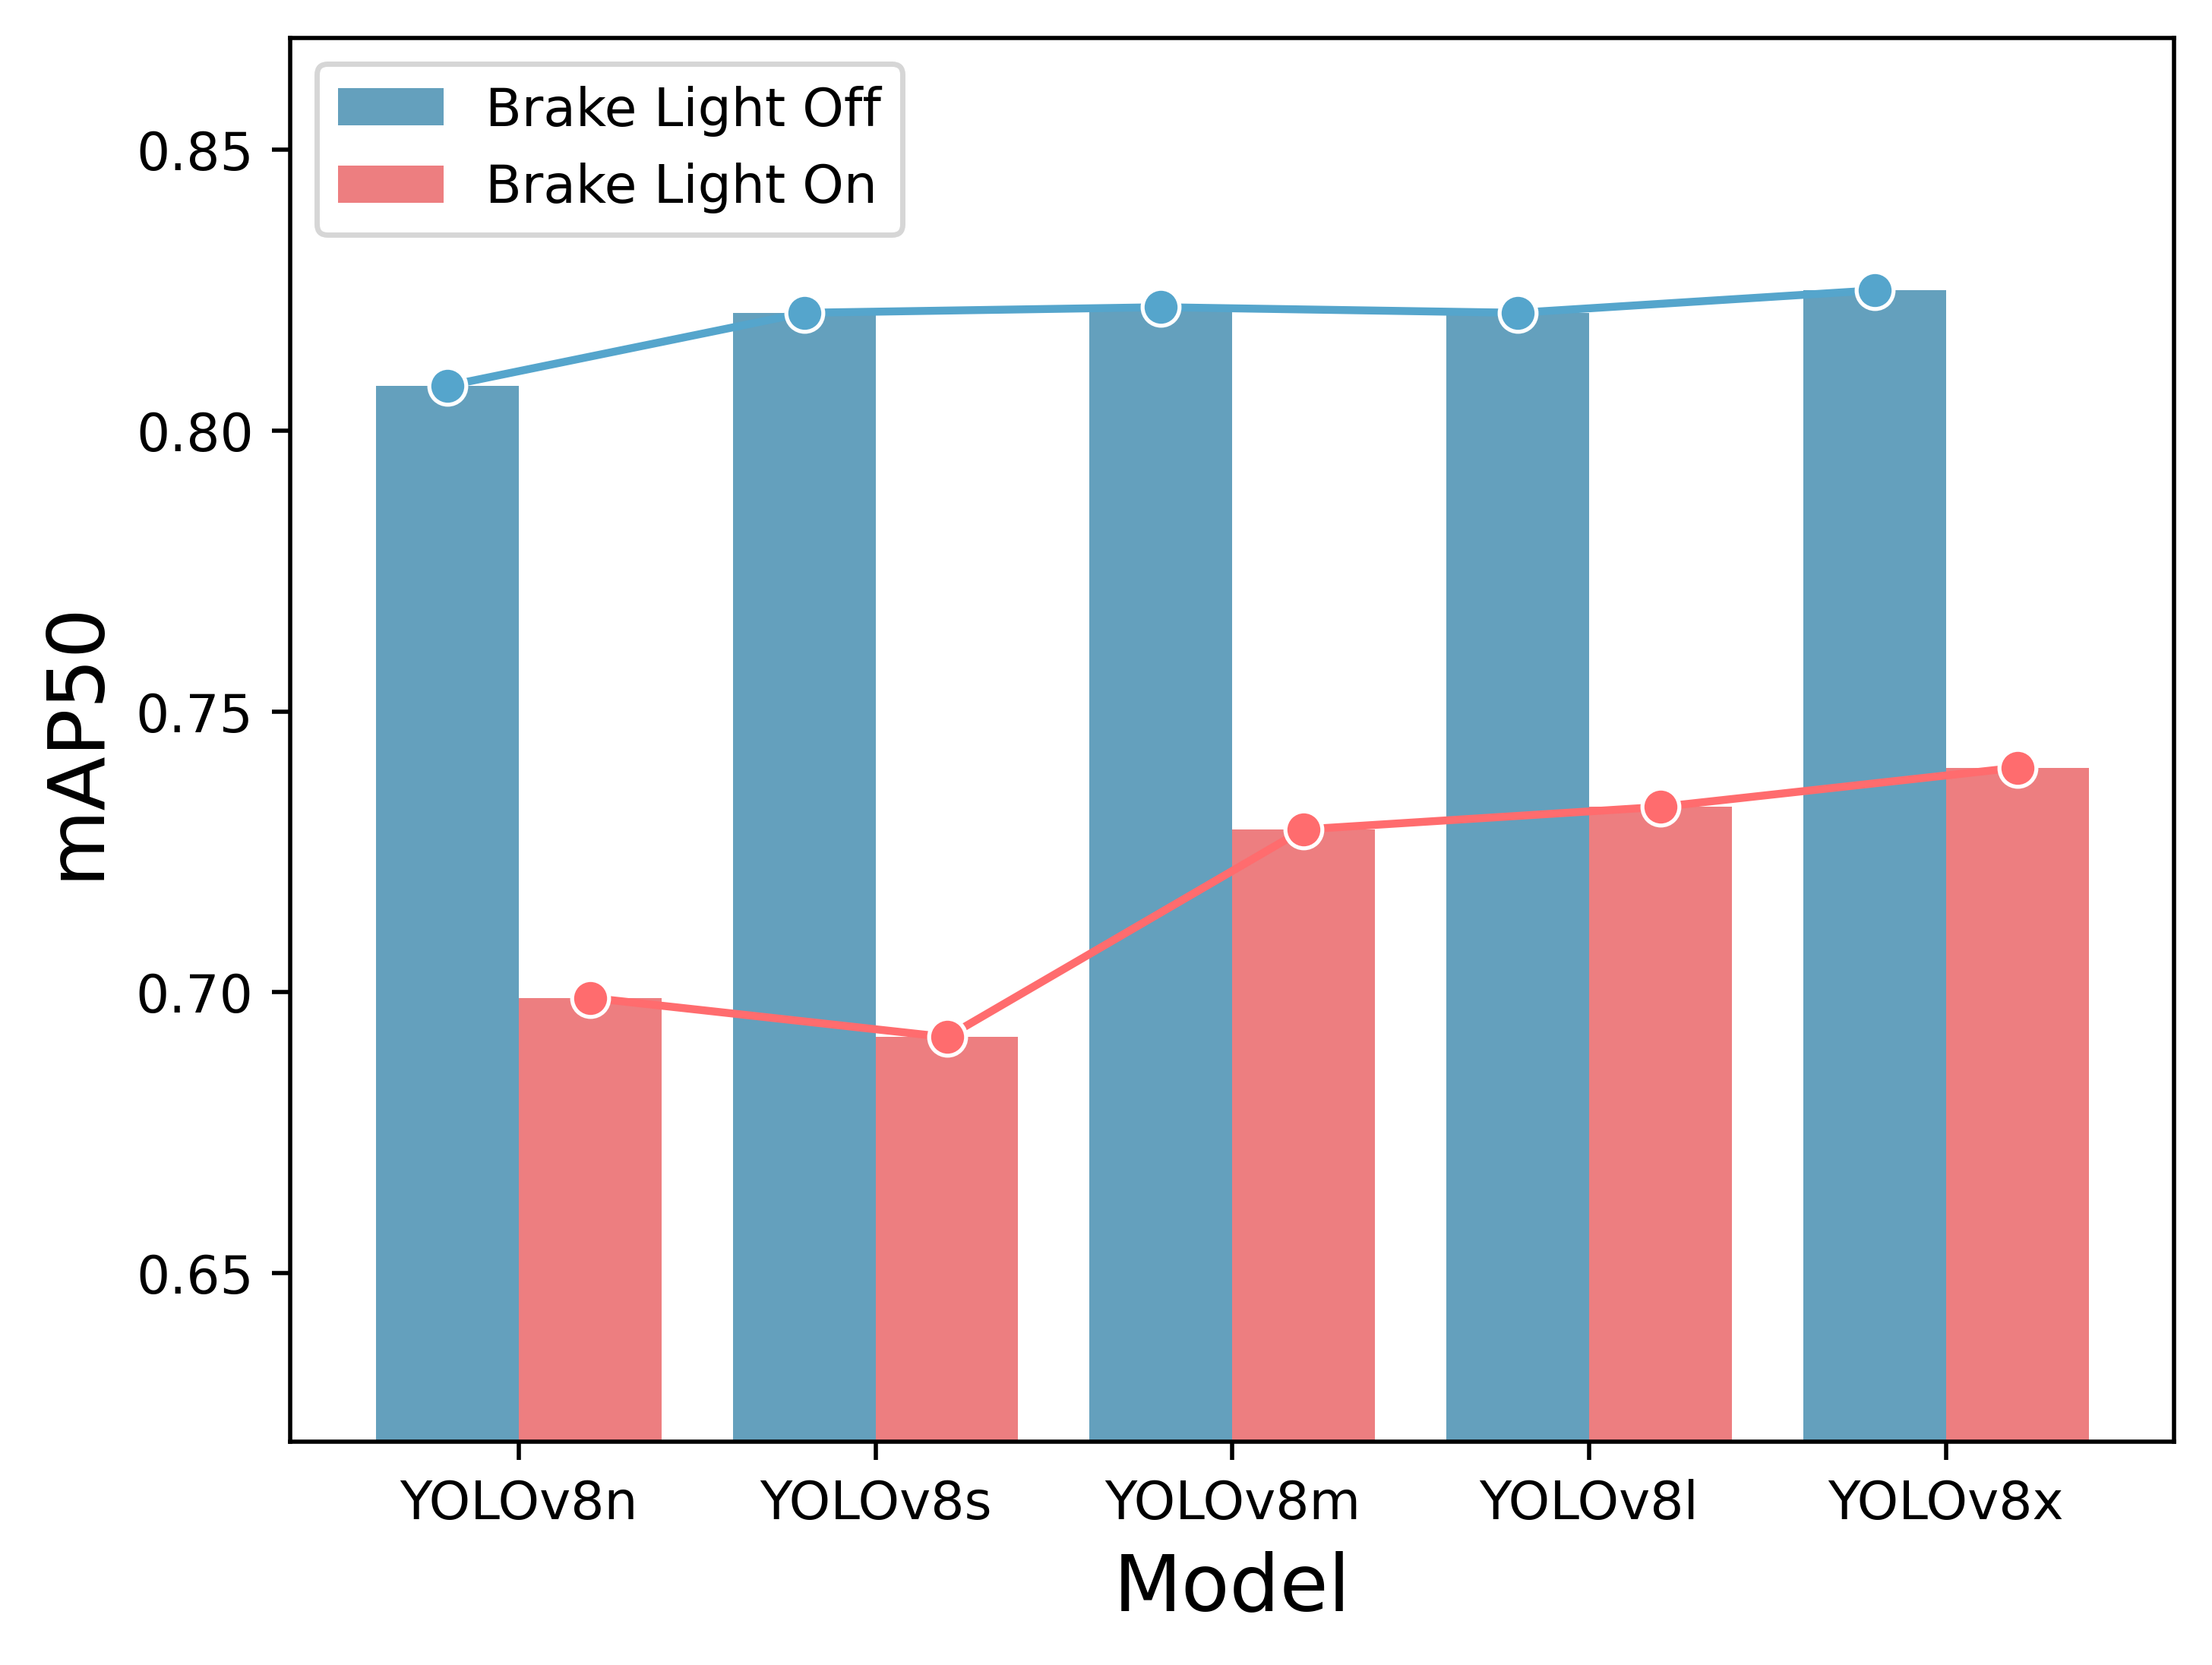
\includegraphics[height=5cm]{fig/bar_day_map50.png} }}%
    \subfloat[mAP50 on the Night testset]{{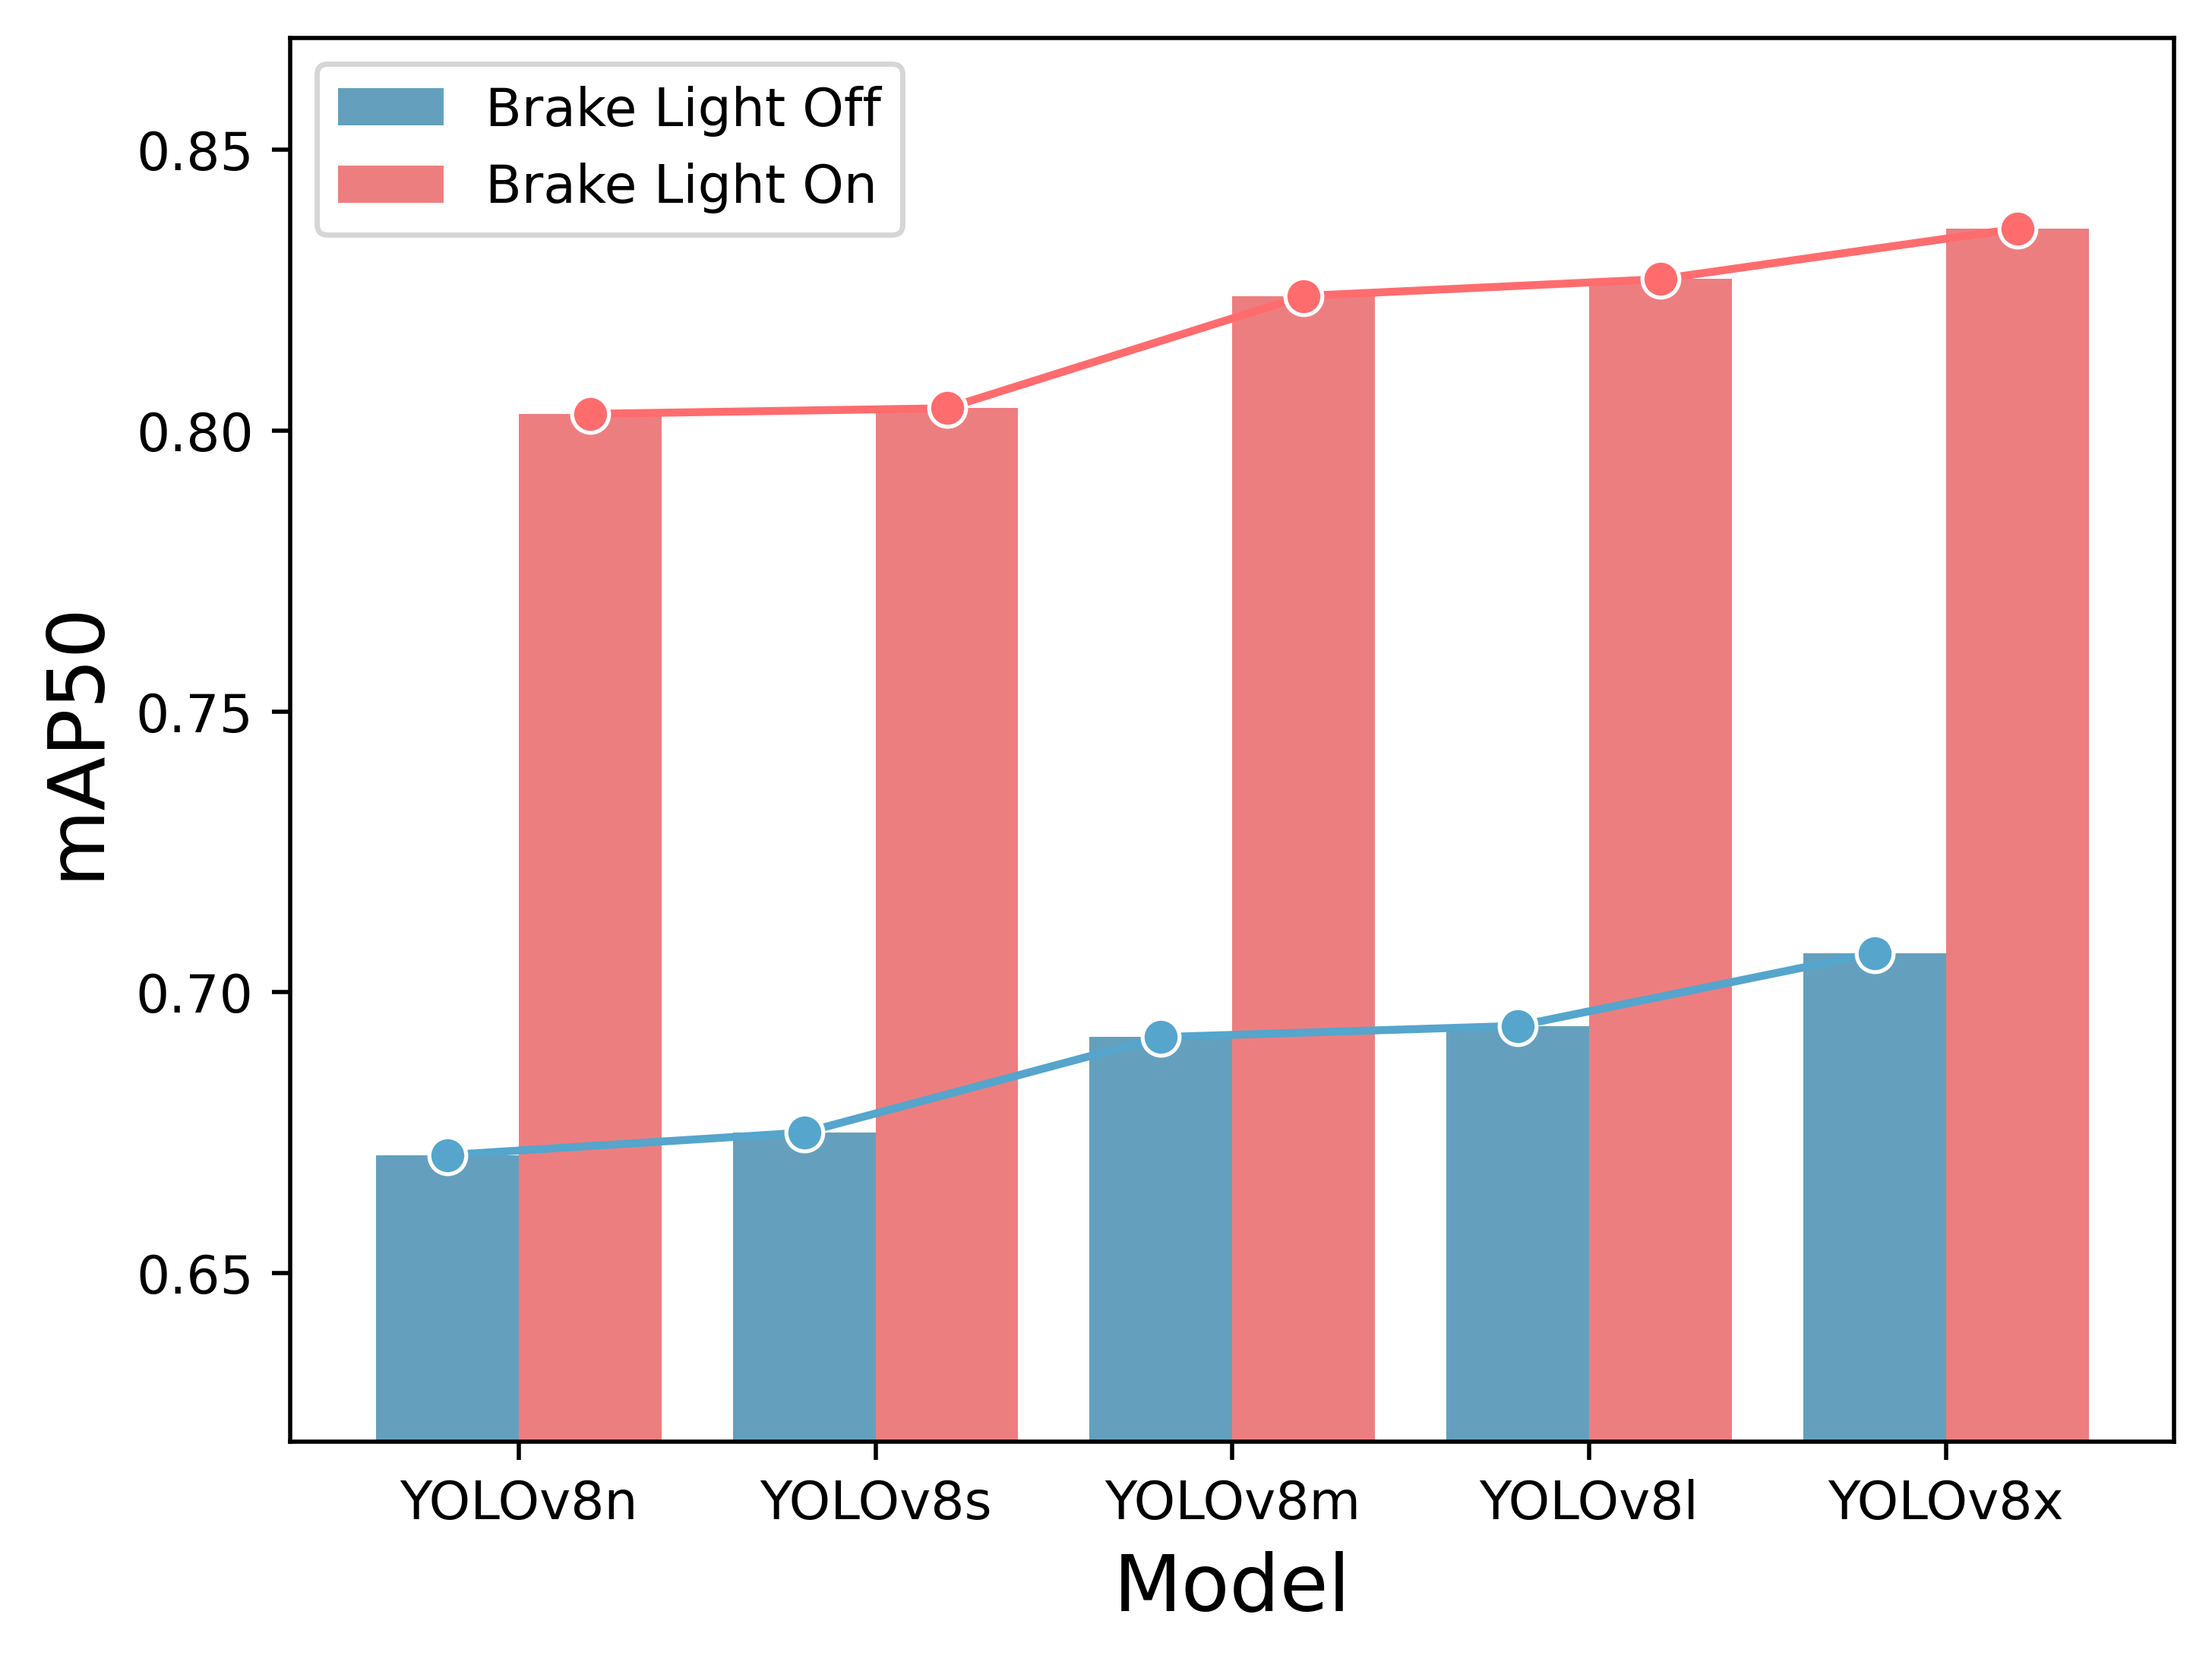
\includegraphics[height=5cm]{fig/bar_night_map50.png} }}%
    \hfill
    \subfloat[mAP50-95 on the Day testset]{{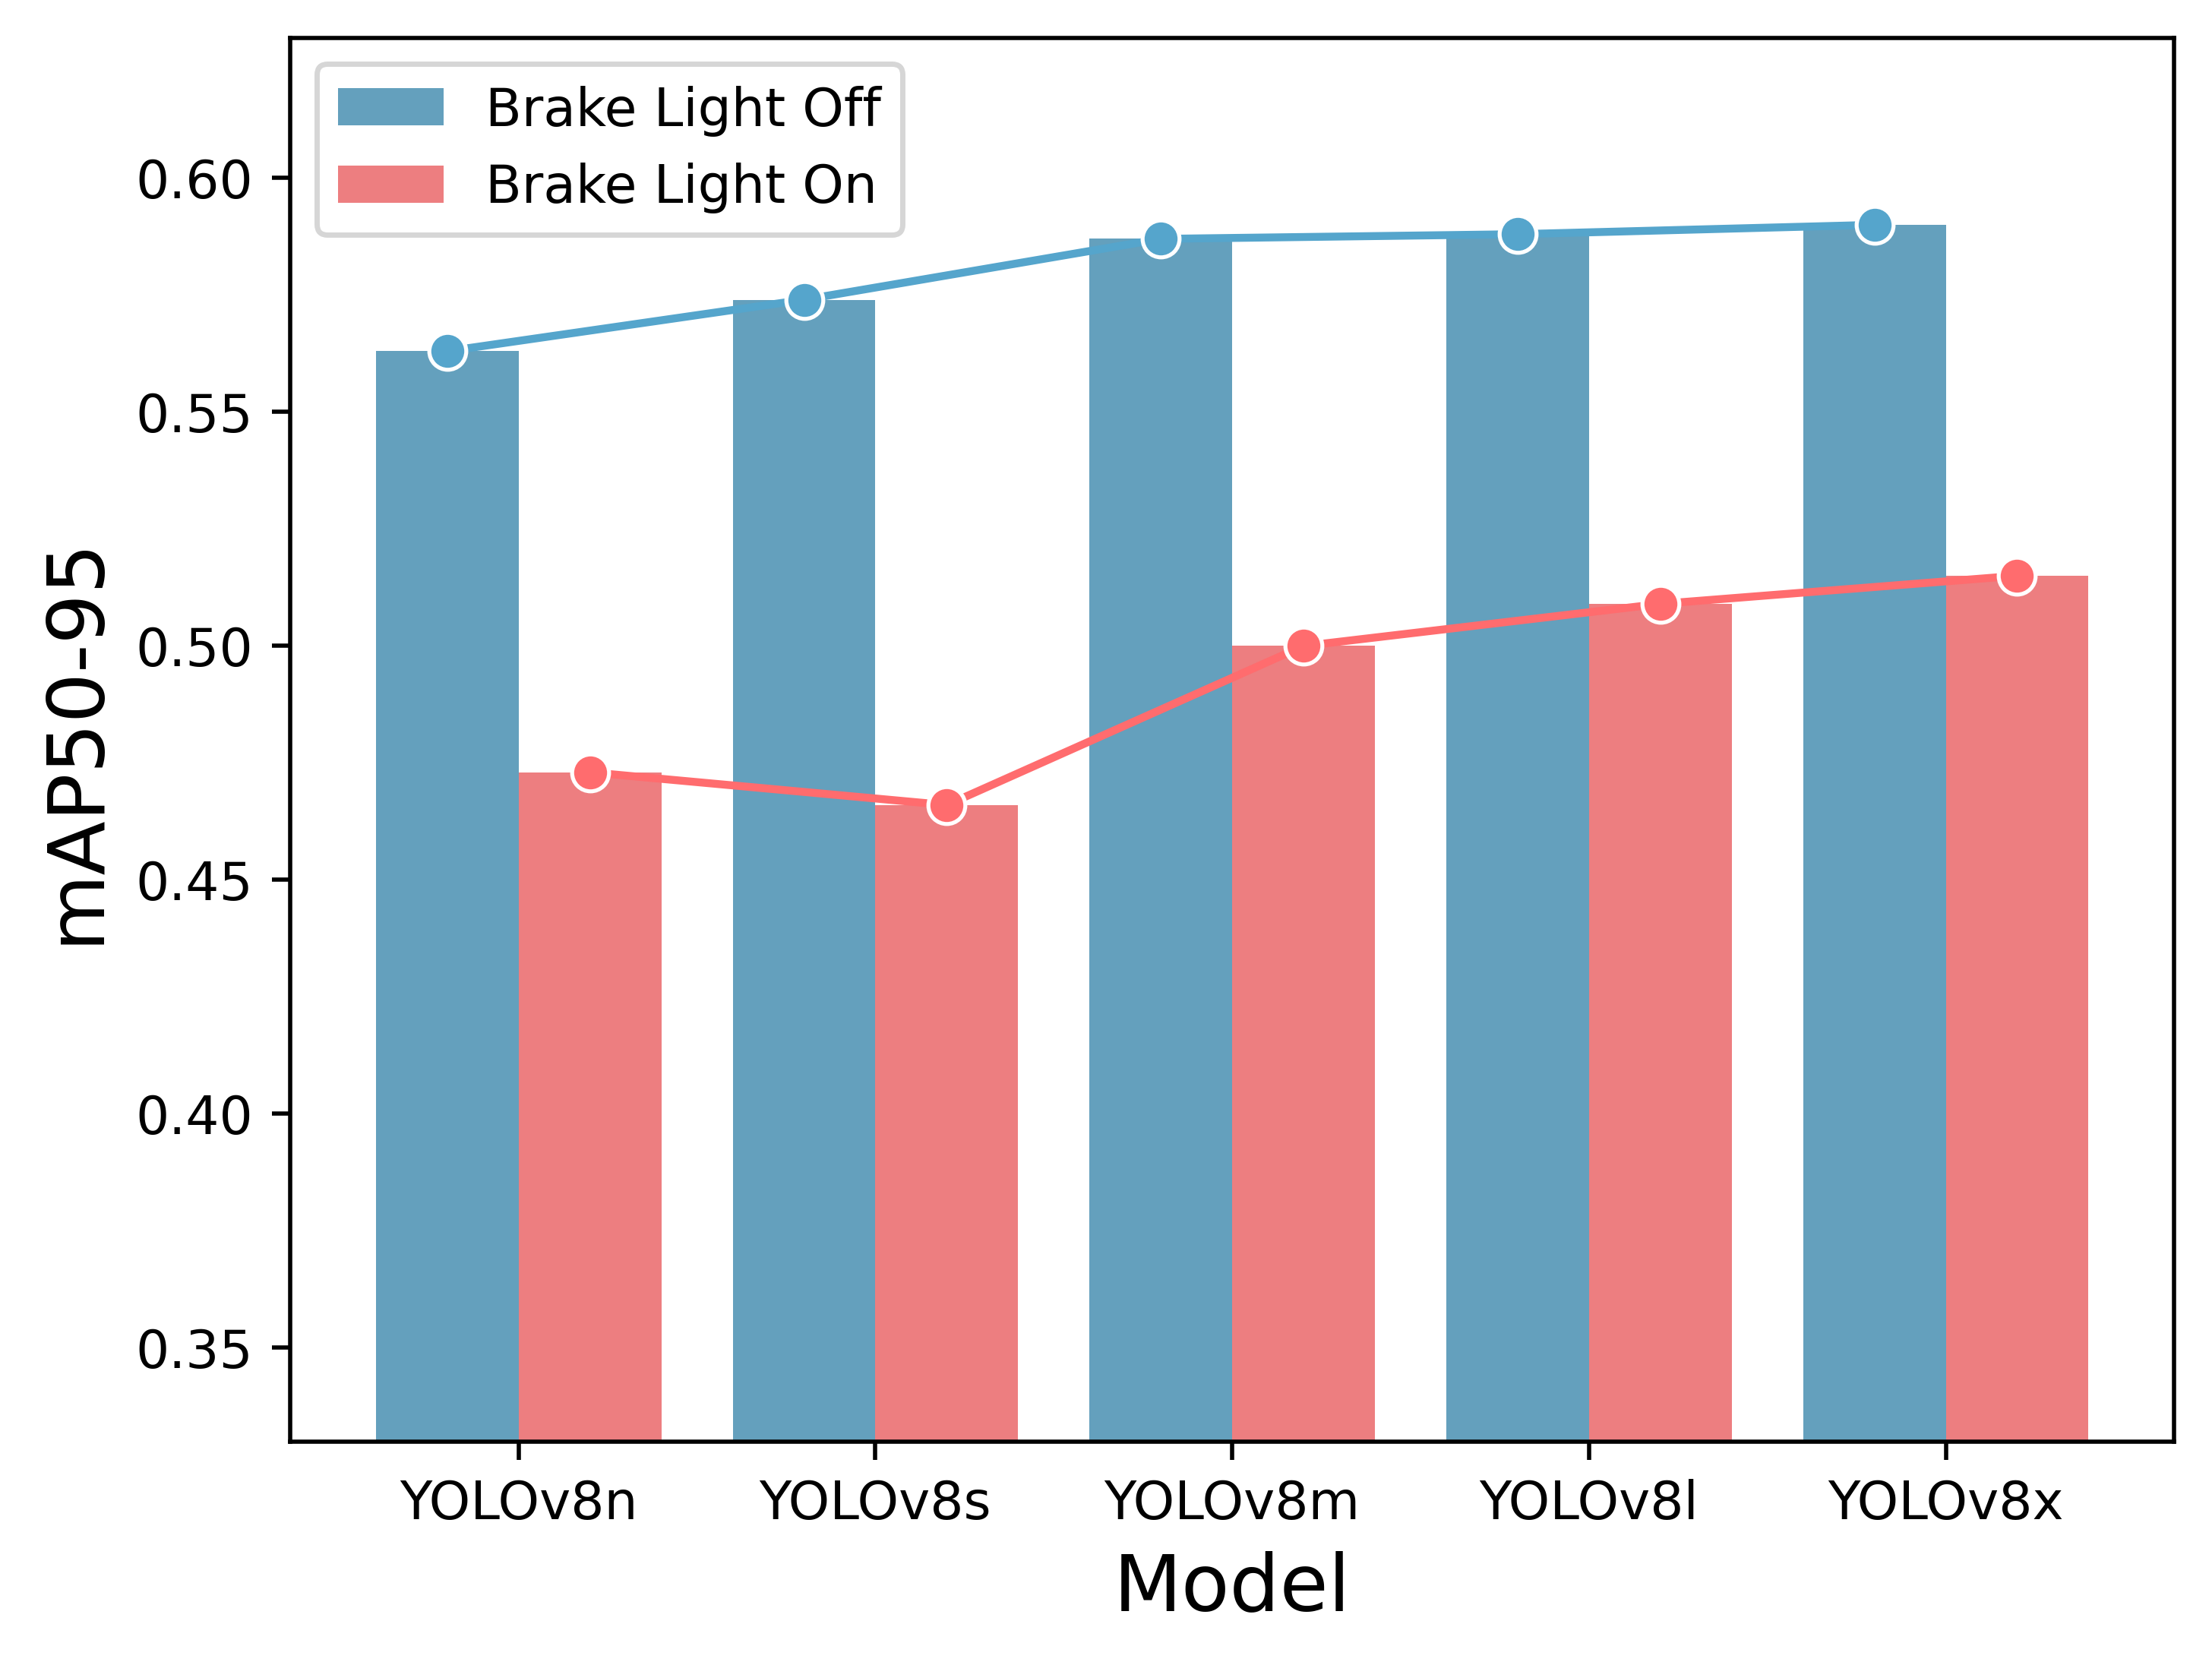
\includegraphics[height=5cm]{fig/bar_day_map50-95.png} }}%
    \subfloat[mAP50-95 on the Night testset]{{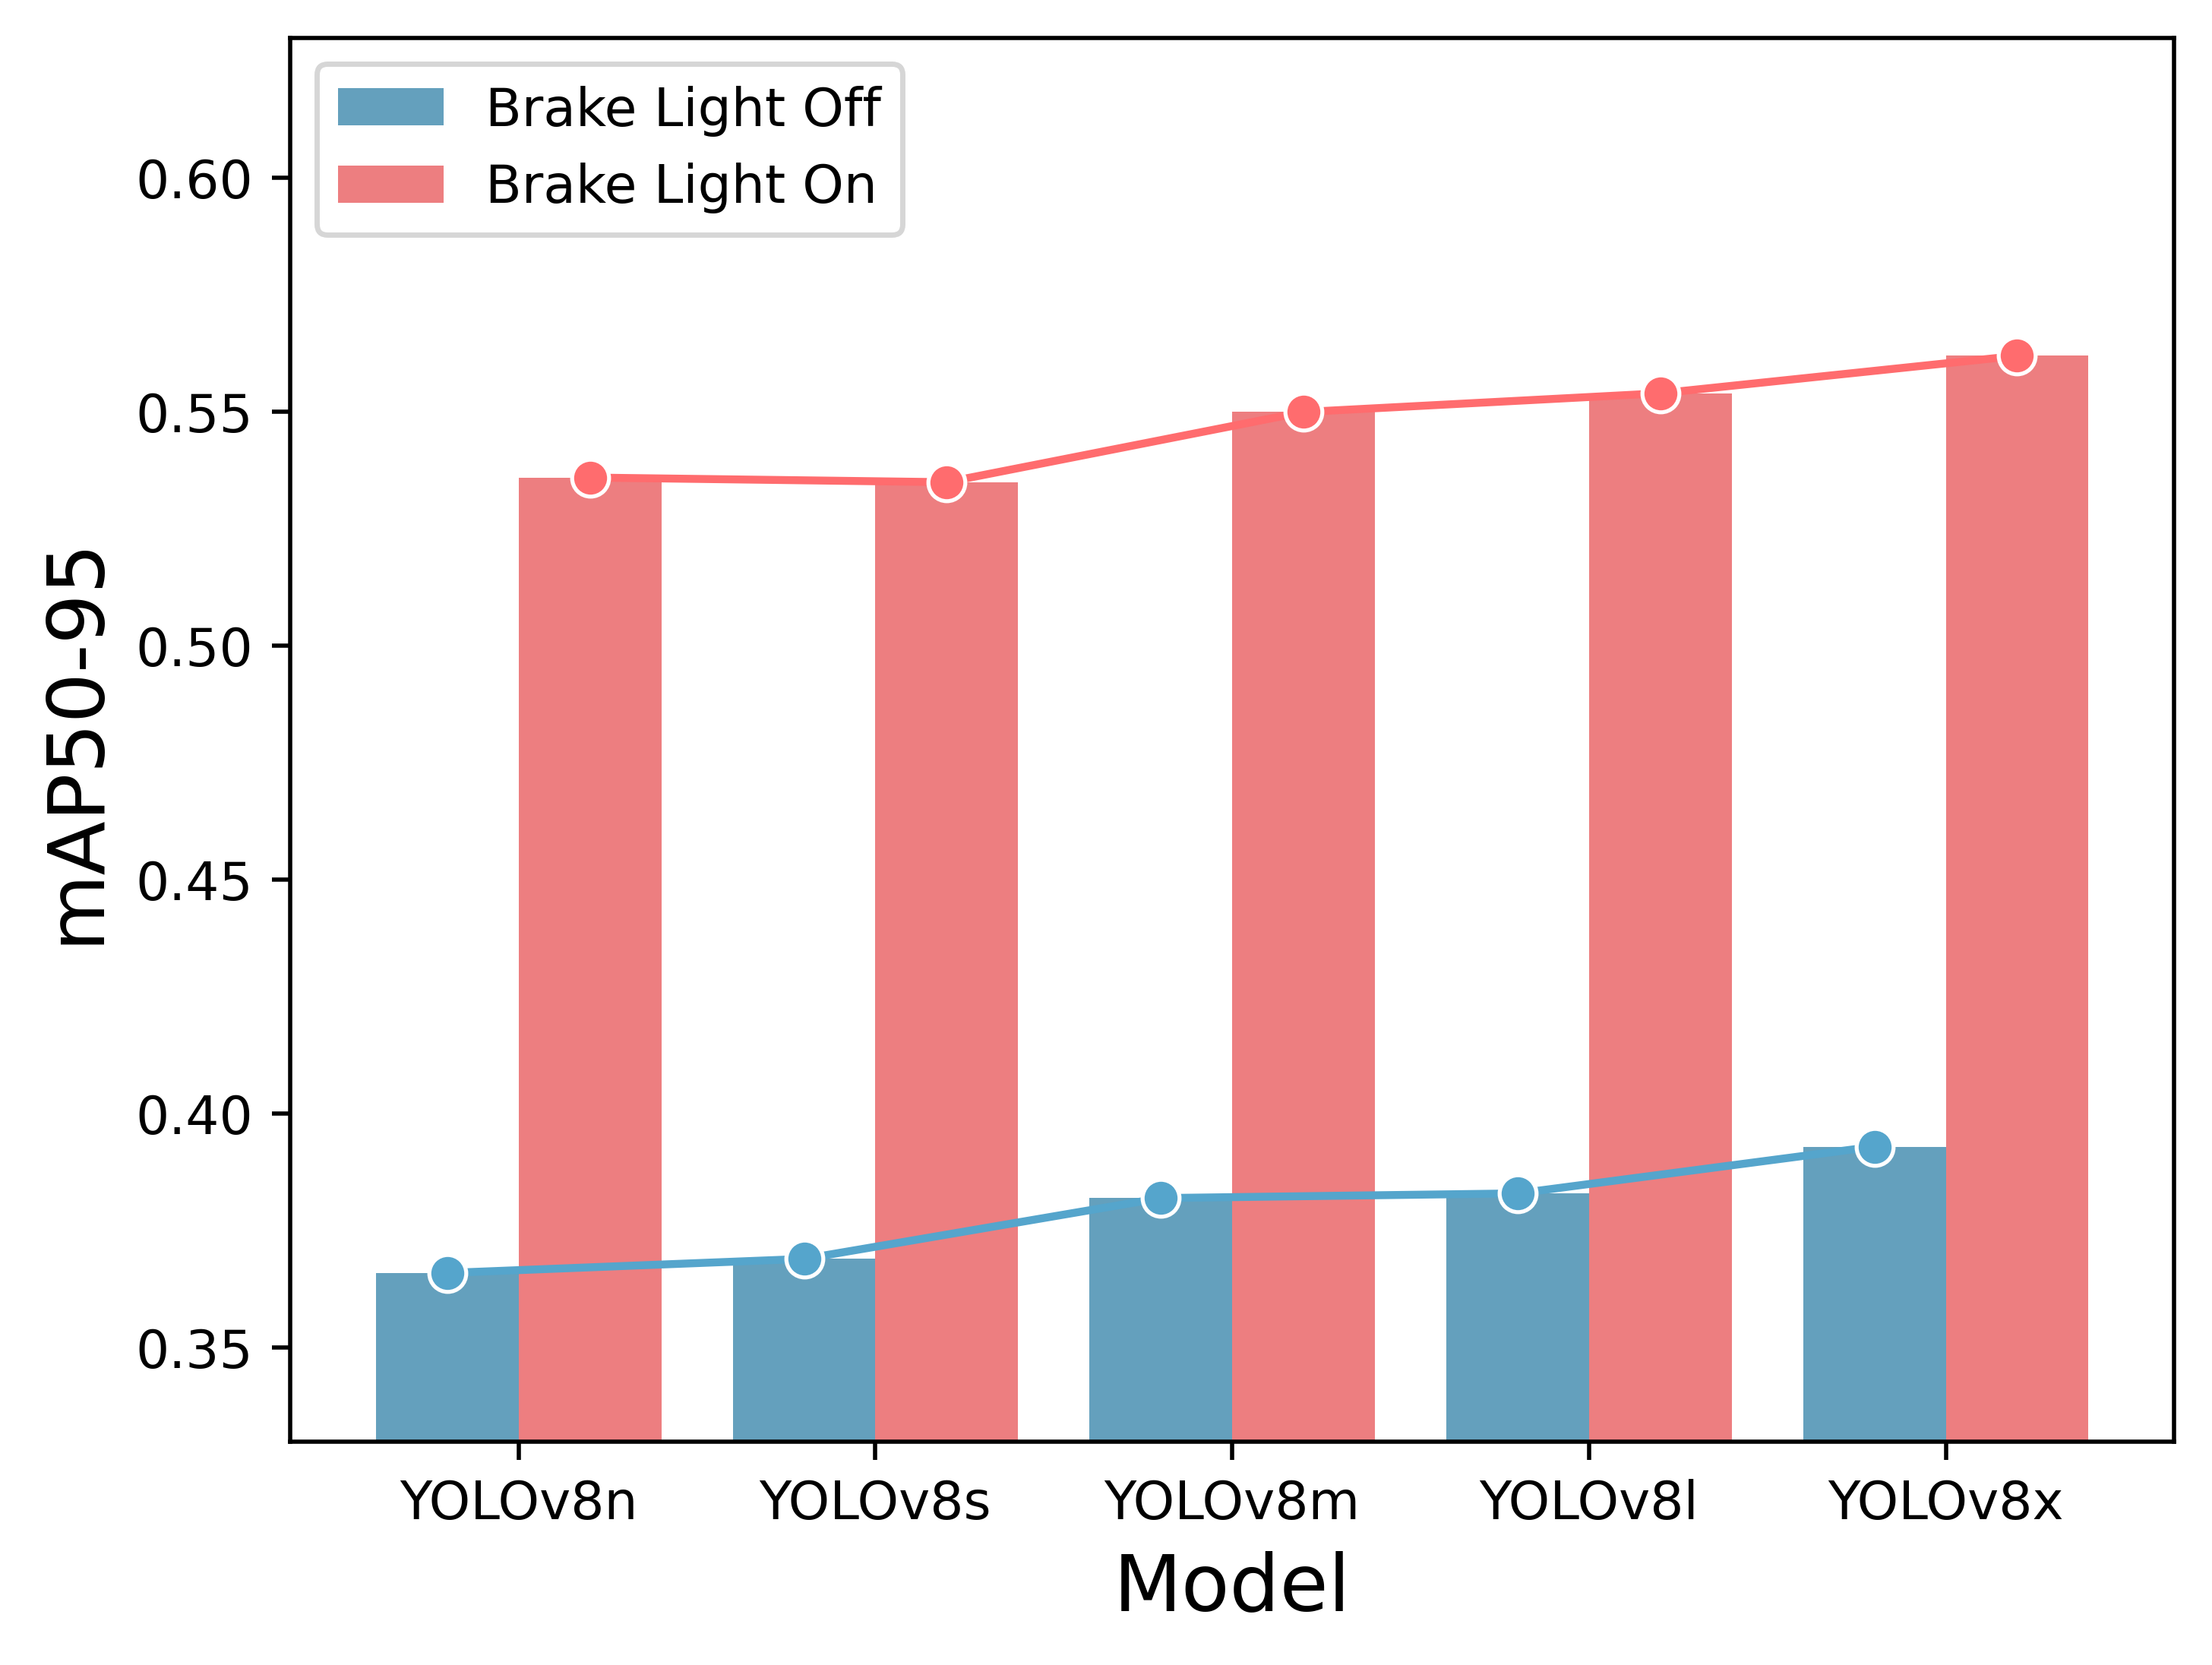
\includegraphics[height=5cm]{fig/bar_night_map50-95.png} }}%

\caption{Detection performance comparison for ambient illumination difference. The y-axis and x-axis represent the detection accuracy and lists the YOLOv8 models, respectively. Each model is depicted with two bars, showcasing the detection performance for brake light off and brake light on classes. Each line plots highlights the difference in detection performance by models for each class.}
\label{fig:dayNnight}%
\end{figure}

In Figure \ref{fig:test_results}, it was observed that the brake light on detection performance for the brake light on class was generally better than that for the brake light off.
However, since the two classes are distinguished solely based on the brightness of the brake light and not the shape or form of the vehicle, it is possible to hypothesize that ambient illumination can affect the detection performance. 
To verify this hypothesis, the test dataset was split into two types based on ambient light levels: Day, representing images taken during daytime with high ambient illumination, and Night, representing images taken at night or in tunnels with low ambient illumination.
The number of images and annotations for each type are provided in Table \ref{tab:test_dataset}.

\begin{table}[h]
    \caption{Details of test dataset}
    \label{tab:test_dataset}
    % \resizebox{\textwidth*0.5}{!}{%
    \begin{tabular}{p{5cm} p{5cm} p{5cm}}
        % {lrr}
    \toprule
    \multicolumn{1}{c}{Number of}                          & \multicolumn{1}{c}{Day} & \multicolumn{1}{c}{Night} \\
    \midrule
    Images                              & \multicolumn{1}{r}{1,467}                     & \multicolumn{1}{r}{1,729}                    \\
    Annotations                         & \multicolumn{1}{r}{4,911}                    & \multicolumn{1}{r}{5,620}                   \\
    \multicolumn{1}{c}{Brake Light Off ($C_{1}=1.0$)} & \multicolumn{1}{r}{3,563}                    & \multicolumn{1}{r}{2,436}                    \\
    \multicolumn{1}{c}{Brake Light On ($C_{2}=1.0$)}  & \multicolumn{1}{r}{1,348}                     & \multicolumn{1}{r}{3,184}                   \\
    \bottomrule
    \end{tabular}%
    % }
\end{table}



Figure \ref{fig:dayNnight} depicts the detection performance for each class on the Day/Night split test dataset. 
In Figure \ref{fig:dayNnight}-(a) and (b), mAP50 is plotted, while in Figure \ref{fig:dayNnight}-(c) and (d), mAP50-95 is plotted.
Figure \ref{fig:dayNnight}-(a) and (c) show the performance on the Day testset, while (b) and (d) show the performance on the Night testset.
On the Day testset, the detection performance for the brake light off class is better than that for the brake light on class.
Conversely, on the Night testset, the detection performance for the brake light on class is superior to that for the brake light off class.
The brake light off class, which was well detected in an environment with high ambient light, experienced a decline in detection performance as the ambient light decreased.
On the other hand, the brake light on class, which initially exhibited relatively low detection performance in an environment with high ambient light, demonstrated high detection performance when the ambient light was low.
The difference in performance due to ambient illumination is more pronounced in the brake light off class.
Detailed detection performance comparisons for ambient illumination difference for each model and class can be found in Table \ref{tab:dayNnight}.


\begin{table}[!h]
    \caption{Results of comparison for ambient illumination difference}
    \label{tab:dayNnight}
    % \resizebox{\textwidth}{!}{%
    \renewcommand{\arraystretch}{0.94}
    \begin{tabular}{llcccc}
    \toprule
    \multicolumn{1}{c}{\multirow{2}{*}{Model}} & \multicolumn{1}{c}{\multirow{2}{*}{Class}} & \multicolumn{2}{c}{mAP50}                           & \multicolumn{2}{c}{mAP50-95}                        \\
    \multicolumn{1}{c}{}                       & \multicolumn{1}{c}{}                       & \multicolumn{1}{c}{Day} & \multicolumn{1}{c}{Night} & \multicolumn{1}{c}{Day} & \multicolumn{1}{c}{Night} \\
    \midrule
    \multirow{3}{*}{YOLOv8n}                   & Brake Light Off                            & 0.808          & 0.671               & 0.563          & 0.366                     \\
    & Brake Light On                             & 0.699                   & 0.803            & 0.473                   & 0.536            \\
    & \multicolumn{1}{r}{Total}                  & 0.753          & 0.737                     & 0.518          & 0.451                     \\

    \midrule
    \multirow{3}{*}{YOLOv8s}                   & Brake Light Off                            & 0.821          & 0.675                     & 0.574          & 0.369                     \\
    & Brake Light On                             & 0.692                   & 0.804            & 0.466                   & 0.535            \\
    & \multicolumn{1}{r}{Total}                  & 0.757          & 0.739                     & 0.520          & 0.452                     \\

    \midrule
    \multirow{3}{*}{YOLOv8m}                   & Brake Light Off                            & 0.822          & 0.692                     & 0.587          & 0.382                     \\
    & Brake Light On                             & 0.729                   & 0.824            & 0.500                   & 0.550            \\
    & \multicolumn{1}{r}{Total}                  & 0.776                   & 0.758                     & 0.544          & 0.466                     \\

    \midrule
    \multirow{3}{*}{YOLOv8l}                   & Brake Light Off                            & 0.821          & 0.694                     & 0.588          & 0.383                     \\
                                           & Brake Light On                             & 0.733                   & 0.827            & 0.509                   & 0.554            \\
                                           & \multicolumn{1}{r}{Total}                  & 0.777          & 0.761                     & 0.549          & 0.468                    \\
    \midrule
    \multirow{3}{*}{YOLOv8x}                   & Brake Light Off                            & 0.825          & 0.707                     & 0.590          & 0.393                     \\
                                           & Brake Light On                             & 0.740                   & 0.836            & 0.515                   & 0.562            \\
                                           & \multicolumn{1}{r}{Total}                  & 0.782          & 0.772                     & 0.552          & 0.477                    \\
    \bottomrule
    \end{tabular}%
    % }
\end{table}



According to the detailed analysis, the performance difference attributed to the difference in ambient illumination can be explained in terms of accuracy.
The overall accuracies for driving vehicle detection across all classes were $0.87$ in the Day testset and $0.89$ in the Night testset.
As the ambient illumination decreased, the accuracy for driving vehicle detection slightly improved.
However, the accuracies for the brake light off class decreased to $0.67$ in the Day testset and $0.43$ in the Night testset, while the accuracies for the brake light on class increased to $0.75$ in the Day testset and $0.86$ in the Night testset.
The detailed analysis revealed that this performance difference is influenced by the presence of tail lights.
% , the cause of the difference in performance due to the difference in ambient illumination is represented by two factors.
% Therefore, as the ambient illumination decreases, the overall detection performance for driving vehicles improves, while the detection performance for the brake light off class deteriorates and the performance for the brake light on class improves.
% We argue that this phenomenon is influenced by the tail light.
As the ambient illumination decreases, the tail lights of the vehicles are turned on, enhancing the detection performance for driving vehicles.
However, the turned-on tail lights can cause confusion with the turned-on brake lights, leading to a decreases in the detection performance for brake light off class.
Consequently, the decrease in ambient illumination improves the detection performance of vehicles with the brake light turned on while deteriorating the detection performance of vehicles with the brake light turned off.


\begin{figure}[!t]
    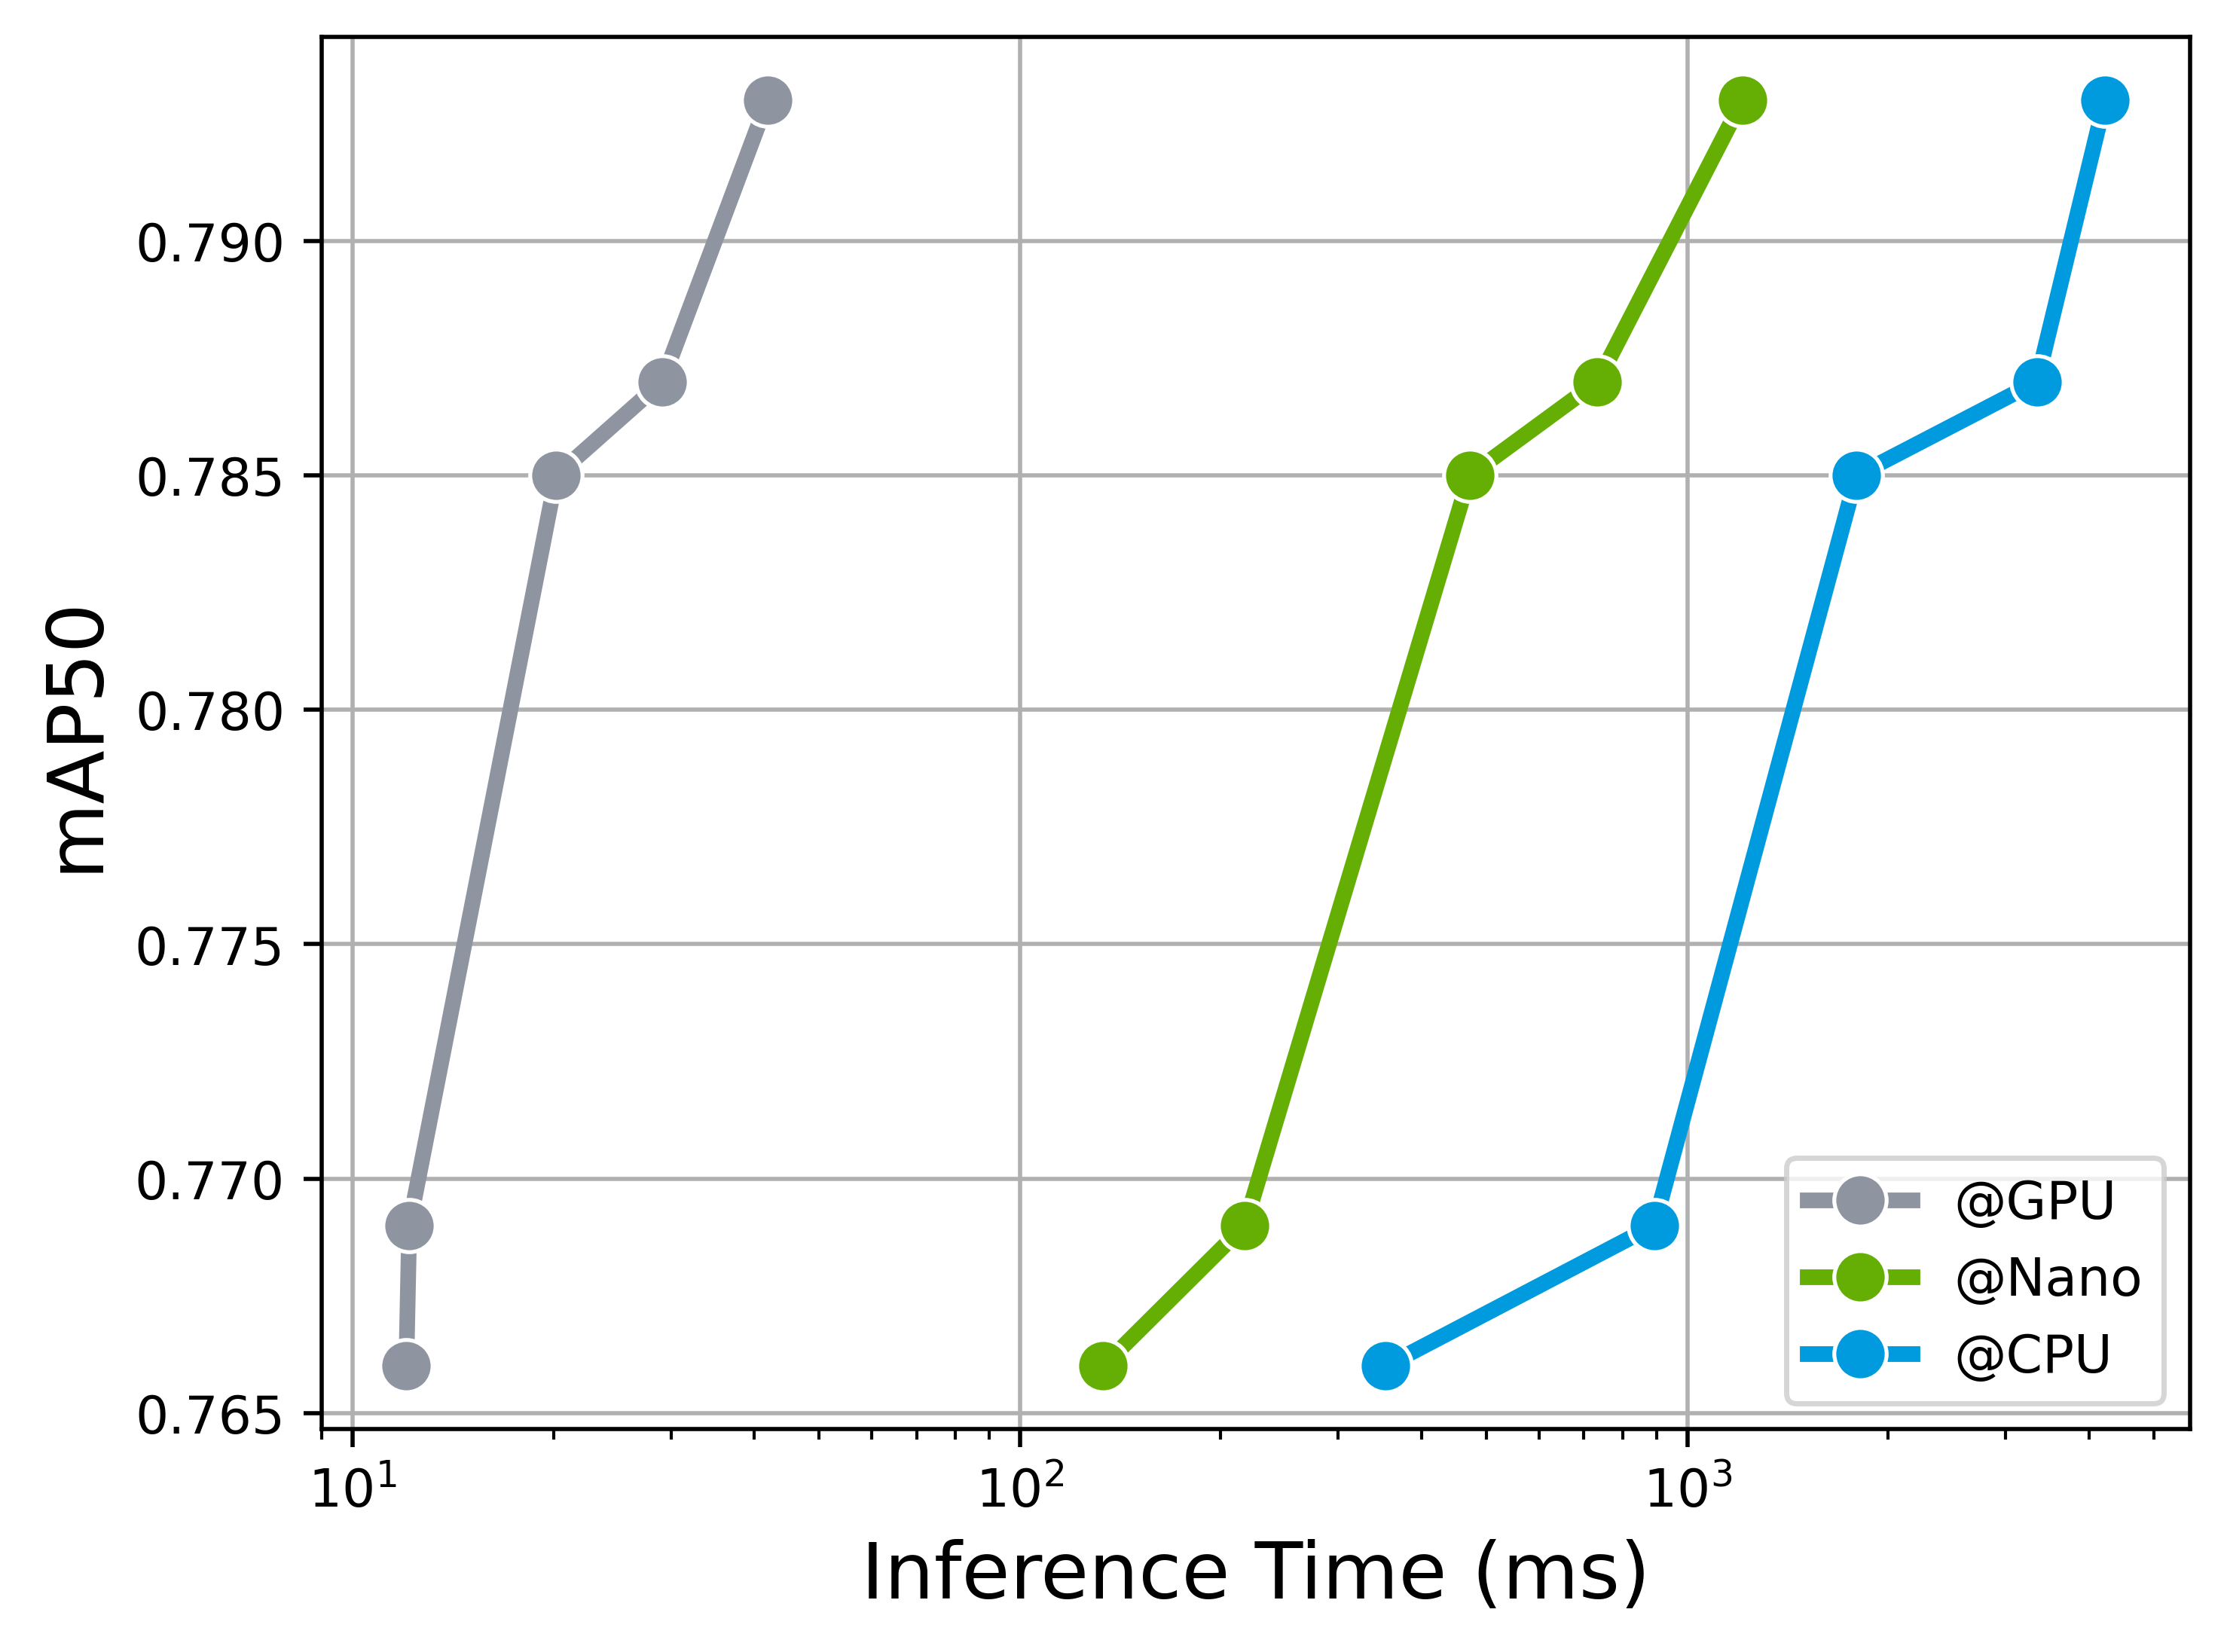
\includegraphics[scale=0.5]{fig/plot_inference_time.png}
    \caption{Trade-off between inference time and detection accuracy in different environments. The x-axis represents the inference time and the y-axis represents the detection accuracy as mAP50. It showcases the trends in inference speed and detection performance for differenct sizes of YOLOv8 under different computing environments as follows: ``@GPU'' refers to Nvidia Tesla T4, ``@Nano'' refers to Nvidia Jetson Nano, and ``@CPU'' refers to Intel Xeon processor.}
    \label{fig:inference}
\end{figure}



In order to validate the real-time inference performance of the trained models on edge devices, experiments were conducted to evaluated both accurate detection and inference time. 
The Nvidia Jetson Nano device was utilized for this purpose.
The trained models were converted to the Open Neural Network Exchange (ONNX) format, which is an open format that facilitates the sharing and interoperability of neural network models across different frameworks. The inference time was measured on the Jetson Nano device using the ONNX models.
The measured inference times ranged from $133.30$ ms to $733.27$ ms, depending on the size of the model.
As expected, among the proposed models, YOLOv8n, with the smallest number of parameters and computations, exhibited the fastest inference time of $133.30$ ms, surpassing even human cognitive processing time.
It is worth noting that the average human cognitive response time is approximately 200 ms.
While faster inference time are generally preferred, it is crucial to acknowledge that Jetson Nano operates in a resource-constrained environment.
Despite these strict limitations, YOLOv8n achieved inference time faster than human cognitive processing, indicating that it is sufficiently real-time capability.
The trade-off performance between inference time and detection accuracy is illustrated in Figure \ref{fig:inference}.
To provide a comprehensive performance comparison, the performance on different devices, including the Jetson Nano, CPU (Intel Xeon 2.20GHz), and GPU (Nvidia Tesla T4), was included.
Detailed values can be found in Table \ref{tab:inference}.

\begin{table}[!h]
    \caption{Results of comparison for inference time in different environments. All models were inferred by converting to ONNX form, and the different computing environments are as follows: ``@GPU'' refers to Nvidia Tesla T4, ``@Nano'' refers to Nvidia Jetson Nano, and ``@CPU'' refers to Intel Xeon processor.}
    \label{tab:inference}
    \begin{tabular}{lrrr}
    \toprule
    \multicolumn{1}{c}{\multirow{2}{*}{Model}}   & \multicolumn{3}{c}{Inference Time (ms)} \\
                                 & ONNX @GPU & ONNX @Nano & ONNX @CPU \\
    \midrule
    YOLOv8n & 12.04        & 133.30            & 353.13    \\
    YOLOv8s & 12.16        & 217.20            & 891.93    \\
    YOLOv8m & 20.20        & 471.59            & 1,792.31   \\
    YOLOv8l & 29.09       & 733.27            & 3,340.26   \\
    YOLOv8x & 41.87       & 1,208.69           & 4,222.87  \\
    \bottomrule
    \end{tabular}%
\end{table}


\begin{table}[!h]
    \caption{Comparison of learning-based brake light status detection algorithms.}
    \label{tab:comparison}
    \resizebox{\textwidth}{!}{%
    \begin{tabular}{lcrrclclc}
        \toprule
        \multicolumn{1}{c|}{\multirow{2}{*}{Study}} & \multicolumn{1}{c|}{\multirow{2}{*}{Proposed work}} & \multicolumn{3}{c|}{Dataset}                                                                                                         & \multicolumn{2}{c}{Brake Light Detection}                       & \multicolumn{2}{|c}{Evaluation}                                                                                    \\
        \multicolumn{1}{c|}{}                       & \multicolumn{1}{c|}{}                               & \multicolumn{1}{c}{\# Data}                                        & \multicolumn{1}{c}{\# Samples} & \multicolumn{1}{c|}{Condition $^{1}$} & \multicolumn{1}{c}{Classification} & Localization & \multicolumn{1}{|c}{Performance} & \multicolumn{1}{c}{Inference time (ms)}                                              \\
        \midrule
        Cui et al. \cite{cui2015vision}                                 & HOG, SVM                                           & 10,000 images                                                      & \multicolumn{1}{r}{-- $^{2}$}          & D                             &  Turned On           &              & 0.75 (Detection rate)           & N/T $^{3}$                                                                             \\
        Nava et al. \cite{nava2019collision}                                & YOLO, SVM                                          & 9,700 images                                                       & 9,700                          & D                             &  Turned On/Off       &              & 0.95 (F1 score)                 & N/T $^{3}$                                                                             \\
        Pirhonen et al. \cite{pirhonen2022brake}                            & YOLOv3, RF                                         & 822 images                                                         & 822                            & D                             &  Turned On/Off       &              & 0.82 (Accuracy)                 & N/T $^{3}$                                                                             \\
        Wang et al. \cite{wang2016appearance}                                & HOG, CNN                                           & 5,600 images                                                       & 5,600                          & D                             &  Turned On           &              & 0.89 (Accuracy)                 & N/T $^{3}$                                                                             \\
        Kim \cite{kim2022detecting}                                        & YOLOv4, CNN, LSTM                                  & 189 videos                                                         & \multicolumn{1}{r}{-- $^{2}$}          & T                             &  Turned On/Off       &              & 0.91 (Accuracy)                 & N/T $^{3}$                                                                             \\
        Li et al. \cite{li2020highly}                                 & YOLOv3 tiny (w/SPP)                                & 4,618 images   & 15,197                         & D, N                          &  Turned On           & \checkmark            & 0.89 (mAP50)                    & 15.87 (GTX-1060)                                                                \\
        \midrule
        \textbf{Ours}                                       & YOLOv8n                                            & 11,088 images & 30,444                         & D, N, T                       &  Turned On/Off       & \checkmark            & 0.76 (mAP50)                     & \begin{tabular}[c]{@{}c@{}}12.04 (Tesla T4)\\ 133.30 (Jetson Nano)\end{tabular} \\
        \bottomrule
    \multicolumn{9}{l}{$^{1}$ The abbreviations for condition mean the following respectively: D=Daytime, N=Nighttime, T=Tunnel.}\\
    \multicolumn{9}{l}{$^{2}$ -- = Not reported.}\\
    \multicolumn{9}{l}{$^{3}$ N/T = Not Tested.}
    \end{tabular}
    }
\end{table}

Table \ref{tab:comparison} provides a detailed description of the differences between our proposed model and the key existing brake light status detection studies.
The algorithms listed in Table \ref{tab:comparison} are state-of-the-art learning-based brake light status detection algorithms. 
The five studies listed at the top are divided into two or more stages, involving vehicle localization and classification of brake light status \cite{cui2015vision,nava2019collision,pirhonen2022brake,wang2016appearance,kim2022detecting}.
The methodologies for each stage are sequentially presented under the second column, named proposed work.
It is important to note that these five studies only present evaluation results for brake light status classification, excluding vehicle localization, and hence, the evaluation metrics such as detection rate, F1 score, or accuracy were used to describe the classification performance.
On the other hand, both the algorithms presented by Li et al. \cite{li2020highly} and our proposed algorithm perform vehicle localization and brake light status classification simultaneously in a single-stage process.
The evaluation results provided encompass both vehicle localization and brake light status classification, and mAP50 was used to describe both classification and localization performance.

When comparing the two mAP50 values in the Table \ref{tab:comparison}, Li et al.'s is higher than ours. However, one should be mindful that the number of classification classes and the dataset differ.
The $0.89$ reported by Li et al. \cite{li2020highly} pertains only to the performance considering the turned on brake light status while our $0.76$ accounts for both turned on and off brake light status.
In terms of data and sample size comparison, our research utilized the largest dataset. 
Further more, our dataset includes diverse environmental conditions, including daytime, nighttime, and tunnel scenarios, which were not all simultaneously considered in the other studies.
By integrating this vast amount data of diverse conditions, our experimental results effectively represent a wide range of real-world scenarios.

Among the existing key algorithms in Table \ref{tab:comparison}, the inference time of the algorithms is only presented through the study by Li et al. \cite{li2020highly}, which reported an impressive inference time of $15.87$ ms.
However, it is important to note that their experiments were conducted on a high-performance GPU, GTX-1060, which may have contributed to the rapid inference speed.
In contrast, our study not only utilized powerful GPU but also conducted experiments on edge device with limited resources.
As the experimental environments differed, direct comparison of the inference speeds between the two algorithms is not feasible.
Nonetheless, our study presented the inference time on edge device, showcasing real-time performance. This demonstration yields more practical research results, considering the constraints of edge devices and emphasizing the relevance of our findings for real-world applications.

\section{Conclusions}
\label{sec:conclusions}


% test results 최대 0.787, MS-COCO와 비교했을 때 분류해야하는 클래스의 차이는 있지만 정의된 임무에 대해서 높은 성능이라고 할 수 있다.
In this paper, we proposed an algorithm that utilizes transfer learning with YOLOv8 to detect driving vehicles on the road and their brake light status.
Our proposed approach exhibits novelty in three main aspects.
Firstly, we constructed and publicly released a dataset specifically designed for detecting driving vehicle and brake light status on the road.
While data based training has become relatively easier with advancements in computer technology, acquiring high-quality datasets remains a challenging.
By making the results of all the tasks, including over 16 hours of real-road driving, manual annotation, and preprocessing considering data characteristics and detection objectives, accessible to everyone, we established a foundation for related research.
Secondly, we proposed a one-stage brake light detection network that guarantees both high accuracy and fast inference speed.
The proposed detection network is the results of transfer learning using the introduced dataset with YOLOv8.
This network takes input of a single frontal image of a driving vehicle and detects all driving vehicles in the image, as well as classifies their brake light status as either off or on.
We trained and evaluated models of various sizes and achieved a high accuracy with a maximum mAP50 of $0.793$.
Additionally, we provide detailed analysis results considering various driving environments, such as various in ambient illumination conditions.
Lastly, we validated the real-time capability by examining the inference time of all trained models on Nvidia Jetson Nano devices installed on the driving vehicle.
By comparing the trade-off performance between detection accuracy and inference time, we obtained a fast inference speed of $133.30$ ms along with a detection performance of mAP50 $0.766$.

Through this research, we have proposed the fast and accurate brake light status detection network to make autonomous driving technology safer, more interpretable, and more comfortable.
However, when examining previous research, it is difficult to find empirical studies other than those suggesting that the brake light status detection results improve the ride comfort of ACC \cite{pirhonen2022predictive}.
Therefore, based on the results of this study, we plan to conduct experimental research on the utilization of brake light status detection results for improving the safety, interpretability, and alleviation of motion sickness in autonomous driving systems.


%%%%%%%%%%%%%%%%%%%%%%%%%%%%%%%%%%%%%%%%%%
% \setcounter{section}{-1} %% Remove this when starting to work on the template.
% \section{How to Use this Template}

% The template details the sections that can be used in a manuscript. Note that the order and names of article sections may differ from the requirements of the journal (e.g., the positioning of the Materials and Methods section). Please check the instructions on the authors' page of the journal to verify the correct order and names. For any questions, please contact the editorial office of the journal or support@mdpi.com. For LaTeX-related questions please contact latex@mdpi.com.%\endnote{This is an endnote.} % To use endnotes, please un-comment \printendnotes below (before References). Only journal Laws uses \footnote.

% % The order of the section titles is different for some journals. Please refer to the "Instructions for Authors” on the journal homepage.

% \section{Introduction}

% The introduction should briefly place the study in a broad context and highlight why it is important. It should define the purpose of the work and its significance. The current state of the research field should be reviewed carefully and key publications cited. Please highlight controversial and diverging hypotheses when necessary. Finally, briefly mention the main aim of the work and highlight the principal conclusions. As far as possible, please keep the introduction comprehensible to scientists outside your particular field of research. Citing a journal paper \cite{ref-journal}. Now citing a book reference \cite{ref-book1,ref-book2} or other reference types \cite{ref-unpublish,ref-communication,ref-proceeding}. Please use the command \citep{ref-thesis,ref-url} for the following MDPI journals, which use author--date citation: Administrative Sciences, Arts, Econometrics, Economies, Genealogy, Humanities, IJFS, Journal of Intelligence, Journalism and Media, JRFM, Languages, Laws, Religions, Risks, Social Sciences, Literature.
% %%%%%%%%%%%%%%%%%%%%%%%%%%%%%%%%%%%%%%%%%%
% \section{Materials and Methods}

% Materials and Methods should be described with sufficient details to allow others to replicate and build on published results. Please note that publication of your manuscript implicates that you must make all materials, data, computer code, and protocols associated with the publication available to readers. Please disclose at the submission stage any restrictions on the availability of materials or information. New methods and protocols should be described in detail while well-established methods can be briefly described and appropriately cited.

% Research manuscripts reporting large datasets that are deposited in a publicly avail-able database should specify where the data have been deposited and provide the relevant accession numbers. If the accession numbers have not yet been obtained at the time of submission, please state that they will be provided during review. They must be provided prior to publication.

% Interventionary studies involving animals or humans, and other studies require ethical approval must list the authority that provided approval and the corresponding ethical approval code.
% \begin{quote}
% This is an example of a quote.
% \end{quote}

% %%%%%%%%%%%%%%%%%%%%%%%%%%%%%%%%%%%%%%%%%%
% \section{Results}

% This section may be divided by subheadings. It should provide a concise and precise description of the experimental results, their interpretation as well as the experimental conclusions that can be drawn.
% \subsection{Subsection}
% \subsubsection{Subsubsection}

% Bulleted lists look like this:
% \begin{itemize}
% \item	First bullet;
% \item	Second bullet;
% \item	Third bullet.
% \end{itemize}

% Numbered lists can be added as follows:
% \begin{enumerate}
% \item	First item; 
% \item	Second item;
% \item	Third item.
% \end{enumerate}

% The text continues here. 

% \subsection{Figures, Tables and Schemes}

% All figures and tables should be cited in the main text as Figure~\ref{fig1}, Table~\ref{tab1}, etc.

% \begin{figure}[H]
% 
\includegraphics[width=10.5 cm]{Definitions/logo-mdpi}
% \caption{This is a figure. Schemes follow the same formatting. If there are multiple panels, they should be listed as: (\textbf{a}) Description of what is contained in the first panel. (\textbf{b}) Description of what is contained in the second panel. Figures should be placed in the main text near to the first time they are cited. A caption on a single line should be centered.\label{fig1}}
% \end{figure}   
% \unskip

% \begin{table}[H] 
% \caption{This is a table caption. Tables should be placed in the main text near to the first time they are~cited.\label{tab1}}
% \newcolumntype{C}{>{\centering\arraybackslash}X}
% \begin{tabularx}{\textwidth}{CCC}
% \toprule
% \textbf{Title 1}	& \textbf{Title 2}	& \textbf{Title 3}\\
% \midrule
% Entry 1		& Data			& Data\\
% Entry 2		& Data			& Data \textsuperscript{1}\\
% \bottomrule
% \end{tabularx}
% \noindent{\footnotesize{\textsuperscript{1} Tables may have a footer.}}
% \end{table}

% The text continues here (Figure~\ref{fig2} and Table~\ref{tab2}).

% % Example of a figure that spans the whole page width. The same concept works for tables, too.
% \begin{figure}[H]
% \begin{adjustwidth}{-\extralength}{0cm}
% \centering
% 
\includegraphics[width=15.5cm]{Definitions/logo-mdpi}
% \end{adjustwidth}
% \caption{This is a wide figure.\label{fig2}}
% \end{figure}  

% \begin{table}[H]
% \caption{This is a wide table.\label{tab2}}
% 	\begin{adjustwidth}{-\extralength}{0cm}
% 		\newcolumntype{C}{>{\centering\arraybackslash}X}
% 		\begin{tabularx}{\fulllength}{CCCC}
% 			\toprule
% 			\textbf{Title 1}	& \textbf{Title 2}	& \textbf{Title 3}     & \textbf{Title 4}\\
% 			\midrule
% \multirow[m]{3}{*}{Entry 1 *}	& Data			& Data			& Data\\
% 			  	                   & Data			& Data			& Data\\
% 			             	      & Data			& Data			& Data\\
%                    \midrule
% \multirow[m]{3}{*}{Entry 2}    & Data			& Data			& Data\\
% 			  	                  & Data			& Data			& Data\\
% 			             	     & Data			& Data			& Data\\
%                    \midrule
% \multirow[m]{3}{*}{Entry 3}    & Data			& Data			& Data\\
% 			  	                 & Data			& Data			& Data\\
% 			             	    & Data			& Data			& Data\\
%                   \midrule
% \multirow[m]{3}{*}{Entry 4}   & Data			& Data			& Data\\
% 			  	                 & Data			& Data			& Data\\
% 			             	    & Data			& Data			& Data\\
% 			\bottomrule
% 		\end{tabularx}
% 	\end{adjustwidth}
% 	\noindent{\footnotesize{* Tables may have a footer.}}
% \end{table}

% %\begin{listing}[H]
% %\caption{Title of the listing}
% %\rule{\columnwidth}{1pt}
% %\raggedright Text of the listing. In font size footnotesize, small, or normalsize. Preferred format: left aligned and single spaced. Preferred border format: top border line and bottom border line.
% %\rule{\columnwidth}{1pt}
% %\end{listing}

% Text.

% Text.

% \subsection{Formatting of Mathematical Components}

% This is the example 1 of equation:
% \begin{linenomath}
% \begin{equation}
% a = 1,
% \end{equation}
% \end{linenomath}
% the text following an equation need not be a new paragraph. Please punctuate equations as regular text.
% %% If the documentclass option "submit" is chosen, please insert a blank line before and after any math environment (equation and eqnarray environments). This ensures correct linenumbering. The blank line should be removed when the documentclass option is changed to "accept" because the text following an equation should not be a new paragraph.

% This is the example 2 of equation:
% \begin{adjustwidth}{-\extralength}{0cm}
% \begin{equation}
% a = b + c + d + e + f + g + h + i + j + k + l + m + n + o + p + q + r + s + t + u + v + w + x + y + z
% \end{equation}
% \end{adjustwidth}

% % Example of a page in landscape format (with table and table footnote).
% %\startlandscape
% %\begin{table}[H] %% Table in wide page
% %\caption{This is a very wide table.\label{tab3}}
% %	\begin{tabularx}{\textwidth}{CCCC}
% %		\toprule
% %		\textbf{Title 1}	& \textbf{Title 2}	& \textbf{Title 3}	& \textbf{Title 4}\\
% %		\midrule
% %		Entry 1		& Data			& Data			& This cell has some longer content that runs over two lines.\\
% %		Entry 2		& Data			& Data			& Data\textsuperscript{1}\\
% %		\bottomrule
% %	\end{tabularx}
% %	\begin{adjustwidth}{+\extralength}{0cm}
% %		\noindent\footnotesize{\textsuperscript{1} This is a table footnote.}
% %	\end{adjustwidth}
% %\end{table}
% %\finishlandscape


% Please punctuate equations as regular text. Theorem-type environments (including propositions, lemmas, corollaries etc.) can be formatted as follows:
% %% Example of a theorem:
% \begin{Theorem}
% Example text of a theorem.
% \end{Theorem}

% The text continues here. Proofs must be formatted as follows:

% %% Example of a proof:
% \begin{proof}[Proof of Theorem 1]
% Text of the proof. Note that the phrase ``of Theorem 1'' is optional if it is clear which theorem is being referred to.
% \end{proof}
% The text continues here.

% %%%%%%%%%%%%%%%%%%%%%%%%%%%%%%%%%%%%%%%%%%
% \section{Discussion}

% Authors should discuss the results and how they can be interpreted from the perspective of previous studies and of the working hypotheses. The findings and their implications should be discussed in the broadest context possible. Future research directions may also be highlighted.

% %%%%%%%%%%%%%%%%%%%%%%%%%%%%%%%%%%%%%%%%%%
% \section{Conclusions}

% This section is not mandatory, but can be added to the manuscript if the discussion is unusually long or complex.

% %%%%%%%%%%%%%%%%%%%%%%%%%%%%%%%%%%%%%%%%%%
% \section{Patents}

% This section is not mandatory, but may be added if there are patents resulting from the work reported in this manuscript.

% %%%%%%%%%%%%%%%%%%%%%%%%%%%%%%%%%%%%%%%%%%
% \vspace{6pt} 

%%%%%%%%%%%%%%%%%%%%%%%%%%%%%%%%%%%%%%%%%%
%% optional
%\supplementary{The following supporting information can be downloaded at:  \linksupplementary{s1}, Figure S1: title; Table S1: title; Video S1: title.}

% Only for journal Methods and Protocols:
% If you wish to submit a video article, please do so with any other supplementary material.
% \supplementary{The following supporting information can be downloaded at: \linksupplementary{s1}, Figure S1: title; Table S1: title; Video S1: title. A supporting video article is available at doi: link.}

% Only for journal Hardware:
% If you wish to submit a video article, please do so with any other supplementary material.
% \supplementary{The following supporting information can be downloaded at: \linksupplementary{s1}, Figure S1: title; Table S1: title; Video S1: title.\vspace{6pt}\\
%\begin{tabularx}{\textwidth}{lll}
%\toprule
%\textbf{Name} & \textbf{Type} & \textbf{Description} \\
%\midrule
%S1 & Python script (.py) & Script of python source code used in XX \\
%S2 & Text (.txt) & Script of modelling code used to make Figure X \\
%S3 & Text (.txt) & Raw data from experiment X \\
%S4 & Video (.mp4) & Video demonstrating the hardware in use \\
%... & ... & ... \\
%\bottomrule
%\end{tabularx}
%}

%%%%%%%%%%%%%%%%%%%%%%%%%%%%%%%%%%%%%%%%%%
\authorcontributions{Conceptualization, S.L.; methodology, G.O.; software, G.O.; validation, S.L.; formal analysis, G.O.; investigation, S.L. and G.O.; resources, S.L and G.O.; data curation, G.O.; writing---original draft preparation, G.O.; writing---review and editing, S.L.; visualization, G.O.; supervision, S.L.; project administration, S.L.; funding acquisition, S.L. All authors have read and agreed to the published version of the manuscript.}

% \funding{Please add: ``This research received no external funding'' or ``This research was funded by NAME OF FUNDER grant number XXX.'' and  and ``The APC was funded by XXX''. Check carefully that the details given are accurate and use the standard spelling of funding agency names at \url{https://search.crossref.org/funding}, any errors may affect your future funding.}
\funding{This work was supported partially by Korea Institute of Police Technology (KIPoT) grant funded by the Korea government(KNPA) (No.092021C26S03000, Development of infrastructure information integration and management technologies for real time traffic safety facility operation) and the BK21 Four Program (5199990814084) of the National Research Foundation of Korea (NRF) funded by the Ministry of Education, Korea.}

% \institutionalreview{In this section, you should add the Institutional Review Board Statement and approval number, if relevant to your study. You might choose to exclude this statement if the study did not require ethical approval. Please note that the Editorial Office might ask you for further information. Please add “The study was conducted in accordance with the Declaration of Helsinki, and approved by the Institutional Review Board (or Ethics Committee) of NAME OF INSTITUTE (protocol code XXX and date of approval).” for studies involving humans. OR “The animal study protocol was approved by the Institutional Review Board (or Ethics Committee) of NAME OF INSTITUTE (protocol code XXX and date of approval).” for studies involving animals. OR “Ethical review and approval were waived for this study due to REASON (please provide a detailed justification).” OR “Not applicable” for studies not involving humans or animals.}
\institutionalreview{Not applicable}

% \informedconsent{Any research article describing a study involving humans should contain this statement. Please add ``Informed consent was obtained from all subjects involved in the study.'' OR ``Patient consent was waived due to REASON (please provide a detailed justification).'' OR ``Not applicable'' for studies not involving humans. You might also choose to exclude this statement if the study did not involve humans.

% Written informed consent for publication must be obtained from participating patients who can be identified (including by the patients themselves). Please state ``Written informed consent has been obtained from the patient(s) to publish this paper'' if applicable.}
\informedconsent{Not applicable}

\dataavailability{
    Code used in this study is available at: \url{https://github.com/gsethan17/one-stage-brake-light-status-detection} (accessed on 9 July 2023). The pre-processed train dataset is publicly available \cite{brake-light-detection_dataset}.    
}
% We encourage all authors of articles published in MDPI journals to share their research data. In this section, please provide details regarding where data supporting reported results can be found, including links to publicly archived datasets analyzed or generated during the study. Where no new data were created, or where data is unavailable due to privacy or ethical restrictions, a statement is still required. Suggested Data Availability Statements are available in section ``MDPI Research Data Policies'' at \url{https://www.mdpi.com/ethics}.} 

% Only for journal Nursing Reports
%\publicinvolvement{Please describe how the public (patients, consumers, carers) were involved in the research. Consider reporting against the GRIPP2 (Guidance for Reporting Involvement of Patients and the Public) checklist. If the public were not involved in any aspect of the research add: ``No public involvement in any aspect of this research''.}

% Only for journal Nursing Reports
%\guidelinesstandards{Please add a statement indicating which reporting guideline was used when drafting the report. For example, ``This manuscript was drafted against the XXX (the full name of reporting guidelines and citation) for XXX (type of research) research''. A complete list of reporting guidelines can be accessed via the equator network: \url{https://www.equator-network.org/}.}

% \acknowledgments{In this section you can acknowledge any support given which is not covered by the author contribution or funding sections. This may include administrative and technical support, or donations in kind (e.g., materials used for experiments).}
\acknowledgments{The authors would like to express their gratitude to annotation experts who assisted in providing high-quality annotations for the dataset introduced in this study. It is through their efforts that the authors were able to complete this research.}


% \conflictsofinterest{Declare conflicts of interest or state ``The authors declare no conflict of interest.'' Authors must identify and declare any personal circumstances or interest that may be perceived as inappropriately influencing the representation or interpretation of reported research results. Any role of the funders in the design of the study; in the collection, analyses or interpretation of data; in the writing of the manuscript; or in the decision to publish the results must be declared in this section. If there is no role, please state ``The funders had no role in the design of the study; in the collection, analyses, or interpretation of data; in the writing of the manuscript; or in the decision to publish the results''.} 
\conflictsofinterest{The authors declare no conflict of interest.}

%%%%%%%%%%%%%%%%%%%%%%%%%%%%%%%%%%%%%%%%%%
%% Optional
% \sampleavailability{Samples of the compounds ... are available from the authors.}

%% Only for journal Encyclopedia
%\entrylink{The Link to this entry published on the encyclopedia platform.}

\abbreviations{Abbreviations}{
The following abbreviations are used in this manuscript:\\

\noindent 
\begin{tabular}{@{}ll}
ADAS & Advanced Driver Assistance Systems\\
SAE & Society for Automotive Engineers\\
ACC & Adaptive Cruise Control\\
TTC & Time to Collision\\
RGB & Red-Green-Blue\\
HSI & Hue-Saturation-Intensity\\
HSV & Hue-Saturation-Value\\
SVM & Support Vector Machine\\
CNN & Convolutional Neural Networks\\
LSTM & Long Short-Term Memory\\
HOG & Histogram of Oriented Gradients\\
SSP & Spatial Pyramid Pooling\\
HDR & High Dynamic Range\\ 
LED & Light Emitting Diode\\ 
CIoU & Complete Intersection over Union \\
DFL & Distribution Focal Loss \\
NMS & Non-Maximum Suppression \\
SGD & Stochastic Gradient Descent\\
NAG & Nesterov Accelerated Gradient\\
mAP & mean Average Precision\\
IoU & Intersection over Union\\
ONNX & Open Neural Network Exchange\\
\end{tabular}
}

% %%%%%%%%%%%%%%%%%%%%%%%%%%%%%%%%%%%%%%%%%%
% %% Optional
\appendixtitles{no} % Leave argument "no" if all appendix headings stay EMPTY (then no dot is printed after "Appendix A"). If the appendix sections contain a heading then change the argument to "yes".
\appendixstart
\appendix
% \section[\appendixname~\thesection]{Detail results}
% \label{sec:appendix}
% \subsection[\appendixname~\thesubsection]{}
% The appendix is an optional section that can contain details and data supplemental to the main text---for example, explanations of experimental details that would disrupt the flow of the main text but nonetheless remain crucial to understanding and reproducing the research shown; figures of replicates for experiments of which representative data are shown in the main text can be added here if brief, or as Supplementary Data. Mathematical proofs of results not central to the paper can be added as an appendix.

% Please add the following required packages to your document preamble:








% \begin{table}[H] 
% \caption{This is a table caption.\label{tab5}}
% \newcolumntype{C}{>{\centering\arraybackslash}X}
% \begin{tabularx}{\textwidth}{CCC}
% \toprule
% \textbf{Title 1}	& \textbf{Title 2}	& \textbf{Title 3}\\
% \midrule
% Entry 1		& Data			& Data\\
% Entry 2		& Data			& Data\\
% \bottomrule
% \end{tabularx}
% \end{table}

% \section[\appendixname~\thesection]{}
% All appendix sections must be cited in the main text. In the appendices, Figures, Tables, etc. should be labeled, starting with ``A''---e.g., Figure A1, Figure A2, etc.

%%%%%%%%%%%%%%%%%%%%%%%%%%%%%%%%%%%%%%%%%%
\begin{adjustwidth}{-\extralength}{0cm}
%\printendnotes[custom] % Un-comment to print a list of endnotes

\reftitle{References}

% Please provide either the correct journal abbreviation (e.g. according to the “List of Title Word Abbreviations” http://www.issn.org/services/online-services/access-to-the-ltwa/) or the full name of the journal.
% Citations and References in Supplementary files are permitted provided that they also appear in the reference list here. 

%=====================================
% References, variant A: external bibliography
%=====================================
\bibliography{ref}

%=====================================
% References, variant B: internal bibliography
%=====================================
% \begin{thebibliography}{999}
% % Reference 1
% \bibitem[Author1(year)]{ref-journal}
% Author~1, T. The title of the cited article. {\em Journal Abbreviation} {\bf 2008}, {\em 10}, 142--149.
% % Reference 2
% \bibitem[Author2(year)]{ref-book1}
% Author~2, L. The title of the cited contribution. In {\em The Book Title}; Editor 1, F., Editor 2, A., Eds.; Publishing House: City, Country, 2007; pp. 32--58.
% % Reference 3
% \bibitem[Author3(year)]{ref-book2}
% Author 1, A.; Author 2, B. \textit{Book Title}, 3rd ed.; Publisher: Publisher Location, Country, 2008; pp. 154--196.
% % Reference 4
% \bibitem[Author4(year)]{ref-unpublish}
% Author 1, A.B.; Author 2, C. Title of Unpublished Work. \textit{Abbreviated Journal Name} year, \textit{phrase indicating stage of publication (submitted; accepted; in press)}.
% % Reference 5
% \bibitem[Author5(year)]{ref-communication}
% Author 1, A.B. (University, City, State, Country); Author 2, C. (Institute, City, State, Country). Personal communication, 2012.
% % Reference 6
% \bibitem[Author6(year)]{ref-proceeding}
% Author 1, A.B.; Author 2, C.D.; Author 3, E.F. Title of presentation. In Proceedings of the Name of the Conference, Location of Conference, Country, Date of Conference (Day Month Year); Abstract Number (optional), Pagination (optional).
% % Reference 7
% \bibitem[Author7(year)]{ref-thesis}
% Author 1, A.B. Title of Thesis. Level of Thesis, Degree-Granting University, Location of University, Date of Completion.
% % Reference 8
% \bibitem[Author8(year)]{ref-url}
% Title of Site. Available online: URL (accessed on Day Month Year).
% \end{thebibliography}

% If authors have biography, please use the format below
%\section*{Short Biography of Authors}
%\bio
%{\raisebox{-0.35cm}{\includegraphics[width=3.5cm,height=5.3cm,clip,keepaspectratio]{Definitions/author1.pdf}}}
%{\textbf{Firstname Lastname} Biography of first author}
%
%\bio
%{\raisebox{-0.35cm}{\includegraphics[width=3.5cm,height=5.3cm,clip,keepaspectratio]{Definitions/author2.jpg}}}
%{\textbf{Firstname Lastname} Biography of second author}

% For the MDPI journals use author-date citation, please follow the formatting guidelines on http://www.mdpi.com/authors/references
% To cite two works by the same author: \citeauthor{ref-journal-1a} (\citeyear{ref-journal-1a}, \citeyear{ref-journal-1b}). This produces: Whittaker (1967, 1975)
% To cite two works by the same author with specific pages: \citeauthor{ref-journal-3a} (\citeyear{ref-journal-3a}, p. 328; \citeyear{ref-journal-3b}, p.475). This produces: Wong (1999, p. 328; 2000, p. 475)

%%%%%%%%%%%%%%%%%%%%%%%%%%%%%%%%%%%%%%%%%%
%% for journal Sci
%\reviewreports{\\
%Reviewer 1 comments and authors’ response\\
%Reviewer 2 comments and authors’ response\\
%Reviewer 3 comments and authors’ response
%}
%%%%%%%%%%%%%%%%%%%%%%%%%%%%%%%%%%%%%%%%%%
\PublishersNote{}
\end{adjustwidth}
\end{document}

